\noindent 
\textcolor{blue}{
The focus of these sections will be on explaining and  enumerating the various system constraints presented by an experiment or domain and what are expected or existing algorithms and data representations.  We would like to keep these sections fairly tight ($<$1 page per experiment), so use references generously without much detail on the existing work in the text here.  
}

% \subsection{Domain X (Example)}

% This is an example template of topics to follow to help guide contributors -- example here is modeled after LHC.

% \begin{itemize}
%     \item \textbf{Domain data representation}: e.g. Domain X experiments consist of a number of subdetectors which make frame (event)-based measurements.  Each event is statistically independent.  Different subdetectors measure events in various geometries which can be generically characterized in point clouds...
%     \item \textbf{Experimental challenges and constraints}: Detectors in domain X record data at a rate of 40~MHz.  In order to make data rates manageable, a multi-tier online filtering system is required which processes and reconstructs data in real-time.  In the first tier of processing, ASICs and FPGAs perform on-detector and near-detector hard real-time data compression and feature extraction at latency of less than a microsecond.  In the second tier of filtering, soft real-time processing is performed in more traditional off-the-shelf computing and has the potential deploy coprocessors.  Finally, in offline analysis, future runs of the LHC will require processing exabytes of data...
%     \item \textbf{Existing work and opportunities in ML and outlook}: Machine learning is extensively used in LHC data processing from ... to ... Simulation is also a vital aspect of LHC data analysis and is computationally very expensive.  Accelerating simulation is therefore ...
% \end{itemize}

\subsection{Large Hadron Collider}

The Large Hadron Collider (LHC) at CERN is the world's largest and highest-energy particle accelerator where collisions between bunches of protons occur every 25 ns. To study the products of these collisions, several detectors are located along the ring around the interaction points. The aim of the detectors is to measure with high precision the properties of the Higgs boson~\cite{Aad:2012tfa,Chatrchyan:2012ufa} and to search for new physics phenomena beyond the standard model of particle physics, including the search for a dark matter candidate.
Due to the extreme frequency of 40 MHz at which proton bunches collide, the high multiplicity of secondary particles and the large number of sensors, the detectors have to process and store data at enormous rates. For the two multipurpose experiments, CMS~\cite{Collaboration_2008} and ATLAS~\cite{Collaboration_2008}, comprised of tens of millions of readout channels, these rates are of the order of 100 Tb/s. Processing and storing this data presents severe challenges that are among the most critical for the execution of the LHC physics program. 
The approach implemented by the detectors for data processing consists of an online processing stage, where the event is selected from a buffer and analyzed in real time, and an offline processing stage, in which data have been written to disk and are more thoroughly analyzed with sophisticated algorithms. The online processing system, called the \emph{trigger}, reduces the data rate to a manageable level of 10 Gb /s to be recorded for offline processing. The trigger is typically divided into multiple tiers. Due to the limited size of the on-detector buffers, the first tier (Level-1, L1) utilizes FPGAs and ASICs capable of executing the filtering process with a maximum latency of ${\cal O}(1)~\mu$s as required by the system. At the second stage, the high-level trigger (HLT), data are processed on a CPU-based computing farm located at the experimental site with a latency up to 100 ms. Finally, the complete offline event processing is performed on a globally distributed CPU-based computing grid.

Maintaining the capabilities of this system will become even more challenging in the near future.
In 2027, the LHC will be upgraded to the so-called High-Luminosity LHC (HL-LHC) where each collision will produce 5 to 7 times more particles, ultimately resulting in a total amount of accumulated data that will be one order of magnitude higher than achieved with the present accelerator. At the same time, the particle detectors will be made larger, more granular, and capable of processing data at ever increasing rates. Therefore, the physics reach of the experiments will be limited by the accuracy of algorithms and computational resources. 
Machine learning technologies offer promising solutions in both of these areas, thanks to their capacity of extracting the most relevant information from high-dimensional data and to their highly parallelizable implementation on suitable hardware.
It is expected that this new generation of algorithms, if deployed at all stages of the data processing systems of the LHC experiments, will play a crucial part to maintain, and hopefully even rise, the physics performance accompanied by a more efficient usage of the computing resources.

In the following sections, a few examples of application of machine learning models to physics tasks at the LHC are reviewed together with novel methods for their efficient deployment in both the real-time and offline data processing stages.

\subsubsection{Event reconstruction and simulation}
\label{sec:lhceventreco}

The reconstruction of proton-proton collision events in the LHC detectors involves challenging pattern recognition tasks, given the large number ( ${\cal O}(1000)$ ) of secondary particles produced and the high detector granularity. Specialized detector sub-systems and algorithms are used to reconstruct the different types and properties of particles produced in collisions. For example, the trajectories of charged particles are reconstructed from space point measurements in the inner silicon detectors, and the showers arising from particles traversing the calorimeters are reconstructed from clusters of activated sensors. Traditional algorithms are highly tuned for physics performance in the current LHC collision environment, but are inherently sequential and scale poorly to the expected HL-LHC conditions. It is thus necessary to revisit existing reconstruction algorithms and ensure that both the physics and computational performance will be sufficient. Deep learning solutions are currently being explored for this pattern recognition tasks as a significant speed up can be achieved when harnessing heterogeneous computing and parallelizable and efficient ML that exploits AI-dedicated hardware. In particular, modern architectures such as graph neural networks (GNNs) are being explored for the reconstruction of particle trajectories, showers in the calorimeter as well as of the final individual particles in the event.\\

For the reconstruction of the showers in calorimeters, GNNs have been found to predict the properties of the original incident particle with high accuracy starting from individual energy deposits.
The work in~\cite{Gray:2020mcm} proposes a dynamic graph formulation of pooling to dynamically learn the most important relationships between data via an intermediate clustering and therefore remove the need for predetermined graph structure. When applied to the CMS electromagnetic calorimeter with single detector hits as inputs to predict the energy of the original incident particle a 10\% improvement is found over the traditional approach based on boosted decision trees (BDTs).

GNNs have been explored for a similar calorimeter reconstruction task for the high-granular calorimeters that will replace the current design for HL-LHC.
The task will become even more challenging as such detectors will feature irregular sensor structure and shape (e.g. hexagonal sensor cells for CMS~\cite{collaboration:2017gbu}, high occupancy and an unprecedented number of sensors. For this application, architectures such as \textsc{EdgeConv}~\cite{DBLP:abs-1801-07829} and \textsc{GravNet/GarNet}~\cite{Qasim:2019otl} have shown promising performance in the determination of the properties of single showers yielding  excellent energy resolution and high noise rejection~\cite{Ju:2020xty}. While these preliminary studies were focused on scenarios with low particle multiplicities, the scalability of the clustering performance to more realistic collision scenarios is still a subject of active development.\\
%Given the clear and impactful use cases for GNNs in HEP, the next step is efficient hardware acceleration. However, GNNs pose interesting challenges for FPGA and ASIC based acceleration because of their large, variably sized inputs and outputs, and there is research ongoing~\cite{Duarte:2019fta} to discover proper schemes for optimization.
%A proof-of-concept workflow using the NVidia Triton Inference Server and the \textsc{SONIC} client~\cite{Krupa:2020bwg,Wang:2020fjr} in the CMS software stack is already available.

GNNs have also been extensively studied for charged particle tracking (the task of identifying and reconstructing the trajectories of individual particles in the detector) \cite{exatrk_19,duarte_vlimant, heptrkx,dl_tracking}. The first approaches to this problem typically utilized edge-classification GNNs in a three-step process: graphs are constructed by algorithmically constructing edges between tracker hits in a point cloud, the graphs are processed through a GNN to predict edge weights (true edges that are part of true particle trajectories should be highly weighted and false edges should be lowly rated), and finally, the selected edges are are grouped together to form track candidates. 

There have been several studies building upon and optimizing this initial framework. The ExaTrkX collaboration has demonstrated performance improvements by incorporating a recurrent GNN structure \cite{exatrk_19} and re-embedding graphs prior to training the GNNs \cite{embedding}. Other work has shown that using an Interaction Network architecture \cite{battaglia2016interaction} can substantially reduce the number of learnable parameters in the GNN (IN paper citation); the authors also provide comprehensive comparisons between different graph construction and track building algorithms. Recent work has also explored alternate approaches that combine graph building, gnn inference, and track construction into a single algorithm that is trainable end-to-end; in particular, instance segmentation architectures have generated promising results (Point GNN paper citation).

Much of this work has been conducted using the TrackML dataset \cite{trackml}, which simulates a generalized detector under HL-LHC-like pileup conditions. Quantifying the performance of these GNNs in actual experimental data is an on-going point of study.\\ 

Finally, a novel approach based on GNNs~\cite{Pata:2021oez} has been proposed as alternative solution to the so called particle-flow algorithm that is used by LHC experiments to optimally reconstruct each individual particles produced in a collision by combining information from the calorimeters and the tracker~\cite{Sirunyan:2017ulk}. The new GNN algorithm is found to offer comparable physics performance for charged and neutral hadrons to the existing reconstruction algorithm. At the same time, the inference time is found to scale approximately linearly with the particle multiplicity which is promising for the high-luminosity LHC phase to maintain computing costs in within budget. Further improvement to this original approach are currently under study including an event-based loss such as the object condensation approach. Second, a complete assessment of the physics performance remain to be performed to include reconstruction of rare particles and other corners of the phase space. Finally, it remains to be understood how to optimize and coherently interface this with the ML-based approach proposed for tasks downstream and upstream the particle-level reconstruction.\\

The extraction of results from the LHC data crucially relies on a detailed and precise simulation of the physics of proton-proton collisions and of the response of the detector. In fact, the collected data are typically compared to a reference model, representing the current knowledge, in order to either confirm or disprove it. Numerical models, based on Monte Carlo methods, are used to simulate the interaction between elementary particles and matter, while the Geant4 toolkit is employed to simulate the detectors. These simulations are generally very CPU intensive and requires roughly half of the experiment’s computing resources, with this fraction expected to increase significantly for the HL-LHC. Novel computational methods based on ML are being explored so as to perform precise modelling from particle interactions to detector readouts and response, while maintaining feasible computing budgets for HL-LHC. In particular, numerous work have focused on the usage of generative adversarial networks or other state-of-the-art generative models to replace computationally intensive fragments of MC simulation, such as modeling of electromagnetic showers~\cite{Paganini:2017dwg,Paganini:2017hrr,deOliveira:2017pjk}, reconstruction of jet images~\cite{Musella:2018rdi} or matrix element calculations~\cite{Bendavid:2017zhk}. In addition, the usage of ML generative models on end-to-end analysis-specific fast simulations have also been investigated in the context of Drell-Yan~\cite{Hashemi:2019fkn}, dijet~\cite{DiSipio:2019imz} and W+jets~\cite{Chen:2020uds} production. These case-by-case proposal serve as proof-of-principle examples for complementary data augmentation strategy for LHC experiments.

\subsubsection{Heterogeneous computing}

While state-of-the-art deep learning models are being explored for the computing intensive reconstruction of each collision event at the LHC, their efficient deployment in within the experiments' computing paradigms is still a challenge despite the potential speed up when the inference is executed on suitable AI-dedicated hardware. In order to gain from a parallelizable ML-based translation of traditional and mostly sequential algorithms, a heterogeneous computing architecture needs to be implemented in the experiment infrastructure. For this reason, comprehensive exploration of the use of CPU+GPU~\cite{Krupa:2020bwg} and CPU+FPGA~\cite{Duarte:2019fta,Rankin:2020usv} heterogeneous architectures  was made to achieve the desired acceleration of deep learning inference within the data processing workflow of LHC experiments. These works demonstrated that the acceleration of machine learning inference ``as a service'' represents a heterogeneous computing solution for LHC experiments that  potentially requires minimal modification to the current computing model. In this approach, the ML algorithms are transferred to a co-processor on an independent (local or remote) server by reconfiguring the CPU node to communicate with it through asynchronous and non-blocking inference requests.
With the inference task offloaded on demand to the server,  the CPU can be dedicated to perform other necessary tasks within the event.
As one server can serve many CPUs, this approach has the advantage of increasing the hardware cost-effectiveness to achieve the same throughput when comparing it to a direct-connection paradigm.
It also facilitates the integration and scalability of different type of co-processor devices where the best one is chosen for each task. Finally, the existing open-source frameworks that have been optimized for fast DL on several different types of hardware can be exploited for a quick adaptation in within LHC computing. In particular, the aforementioned works exploit the Nvidia Triton Inference Server in within a custom framework, so called Services for Optimized Network Inference on Co-processors (SONIC), to enable remote gRPC calls to either GPUs or FPGAs in within the experimental software which only has to handle the inputs and outputs conversion between event data format and inference server format. The integration of this approach in within the CMS reconstruction software has been shown to lead to a significant overall reduction in the computing demands both at HLT and offline.

\subsubsection{Real-time analysis at 40 MHz}
% Thea: Adding only plots/figures related to talks given at the FastML 2020 workshop, but do discuss other applications.
Bringing deep learning algorithms to the Level-1 hardware trigger is an extremely challenging task due to the strict latency requirement and the resource constraints imposed by the system. Depending on which part of the system an algorithm is designed to run on, a latency down to ${\cal O}(10)~$ns might be required.  With ${\cal O}(100)~$ processors running large-capacity FPGAs, processing thousands of algorithms in parallel, dedicated FPGA-implementations are needed to make ML algorithms as resource-efficient and fast as possible.
To facilitate the design process and subsequent deployment of highly parallel, highly compressed ML algorithms on FPGAs, dedicated open-source libraries have been developed: \hlsfml and \conifer. The former, \hlsfml, provides conversion tools for deep neural networks, while \conifer aids the deployment of Boosted Decision Trees (BDTs) on FPGA. Both libraries, as well as example LHC applications, will be described in the following.
\begin{figure}[htb]
    \centering
    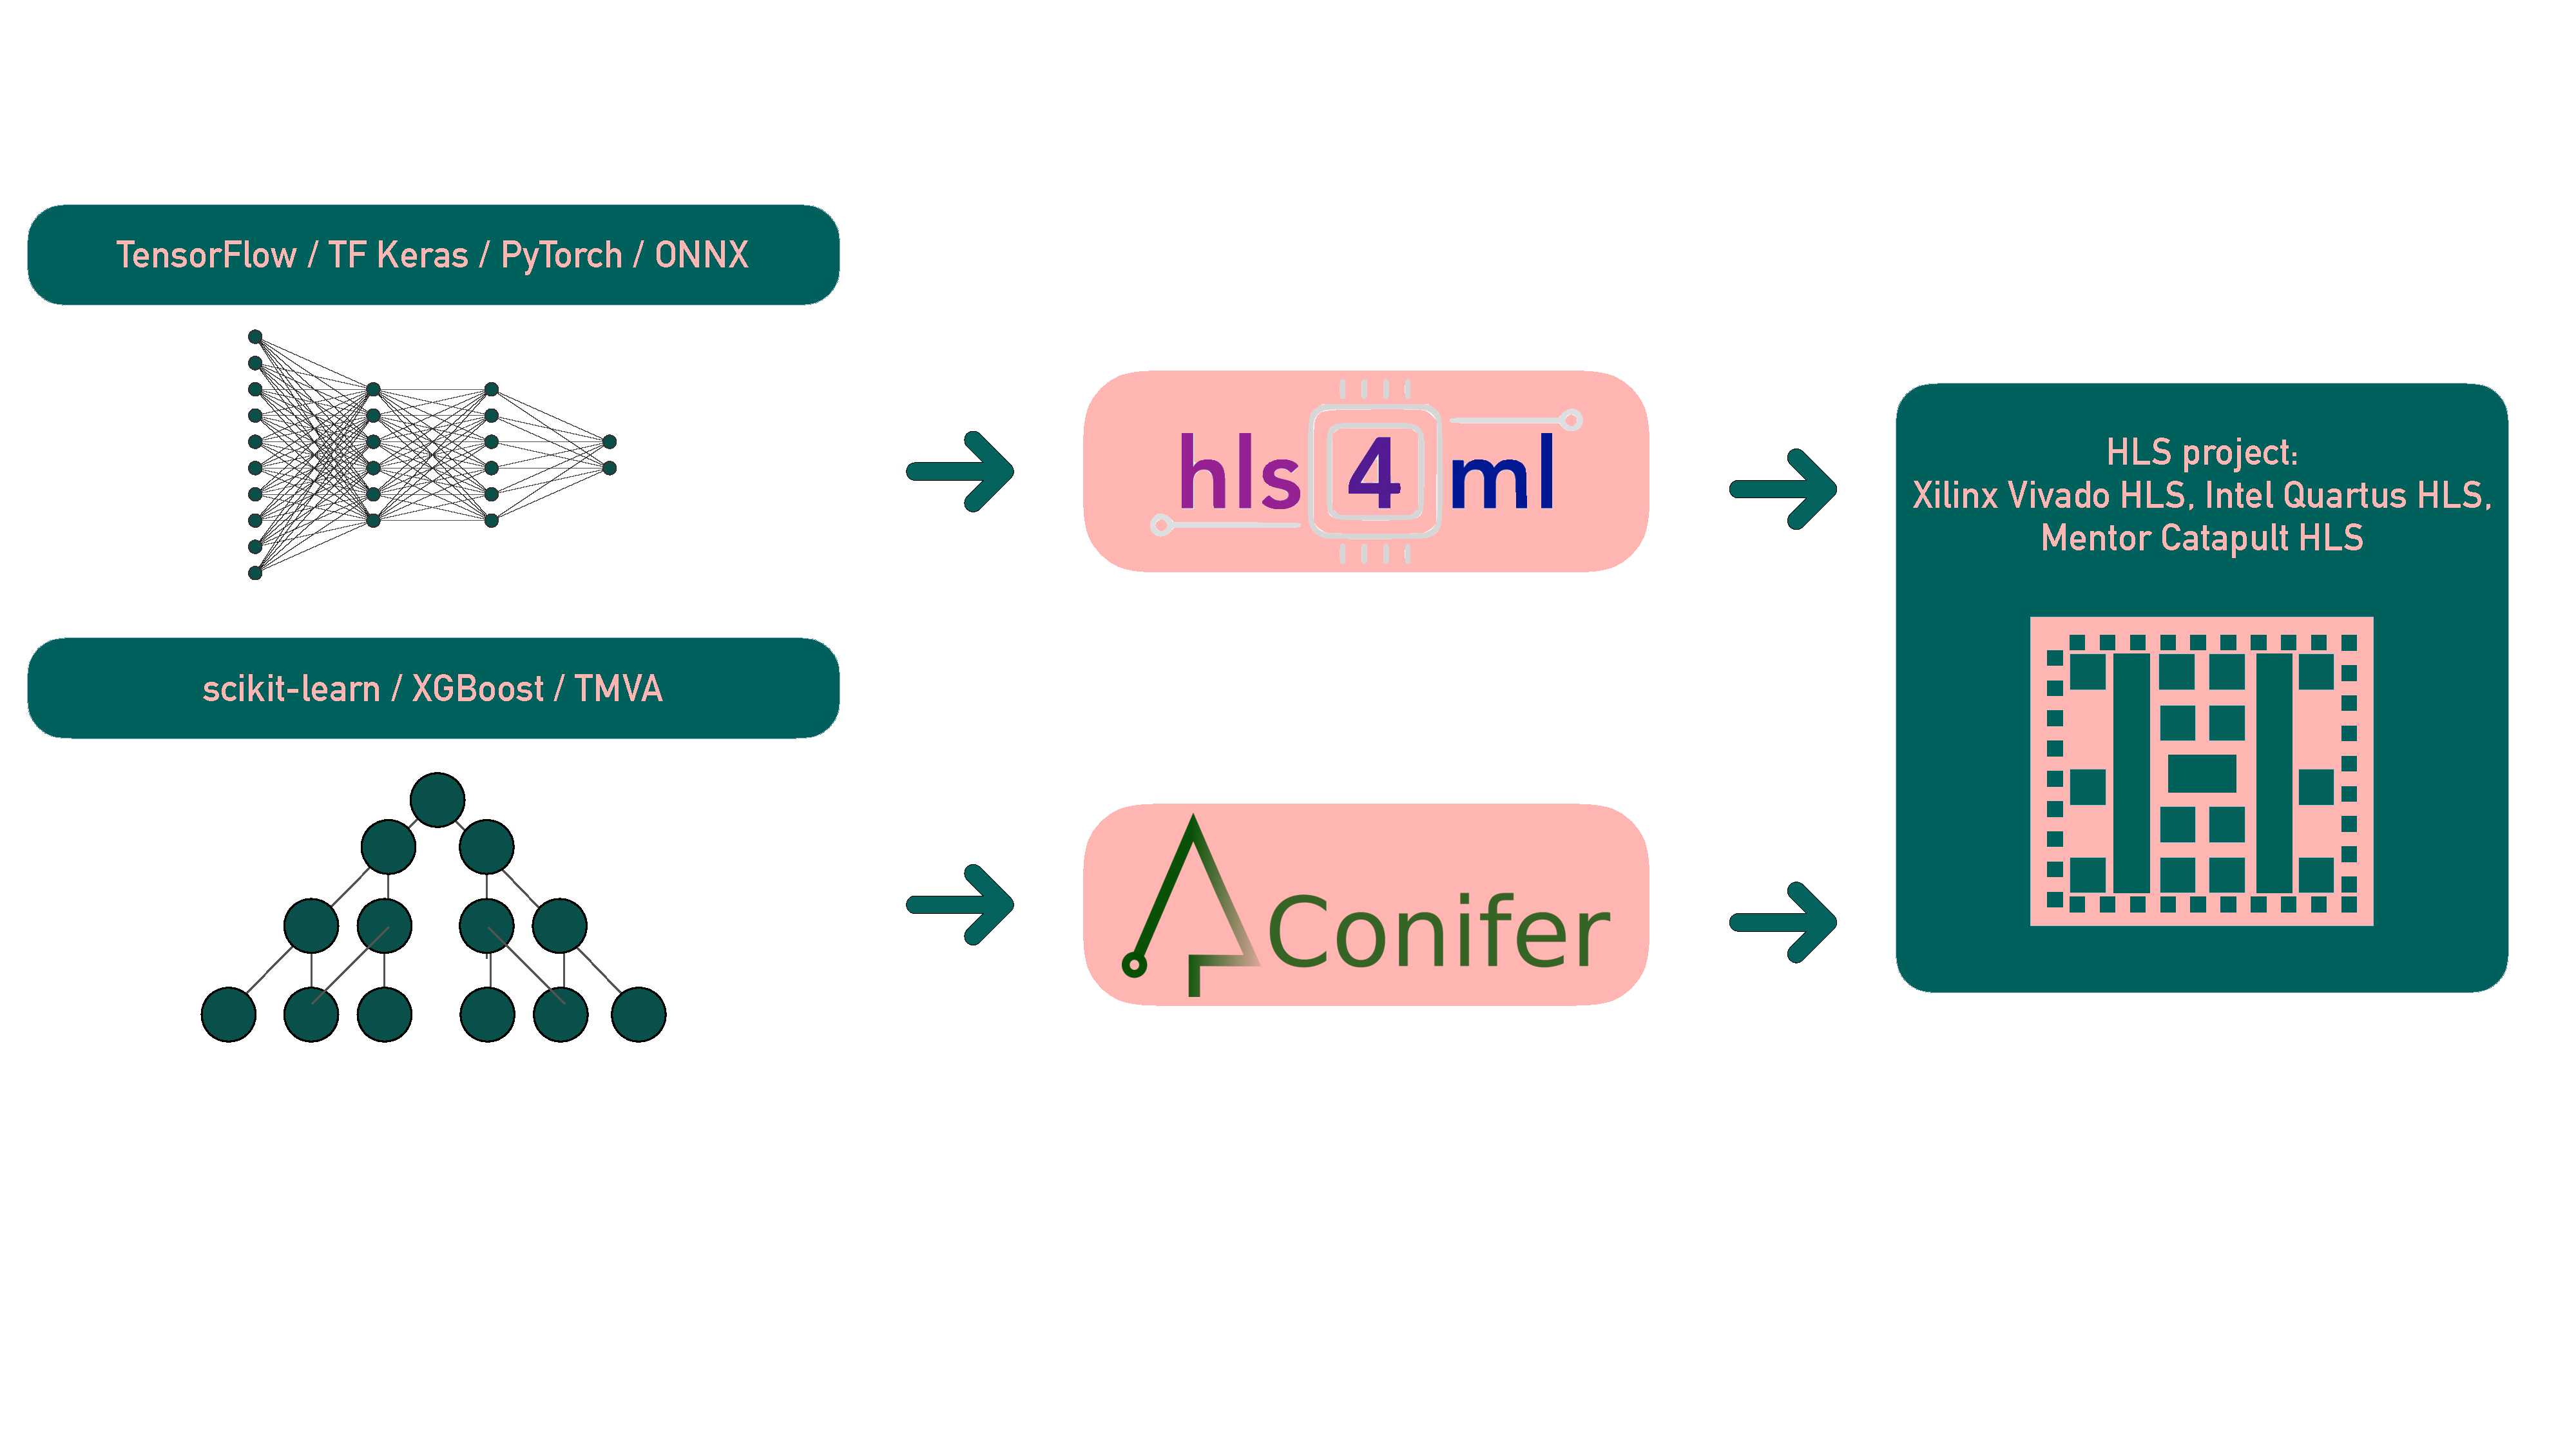
\includegraphics[width=0.89\textwidth]{figures/hls4ml_conifer.pdf}
    \caption{Two dedicated libraries for the conversion of Machine Learning algorithms into FPGA or ASIC firmware: \hlsfml for deep neural network architectures and \conifer for Boosted Decision Tree architectures. Models from a wide range of open-source ML libraries are supported, and may be converted using three different HLS backend.}
    \label{figs2:libraries}
\end{figure}

The \hlsfml library~\cite{Duarte:2018ite,aarrestad2021fast,DiGuglielmo:2020eqx,Coelho:2020zfu} converts pre-trained ML models into ultra low-latency FPGA or ASIC firmware with little overhead required. An integration with the Google QKeras library~\cite{qkeras} allows users to design aggressively quantized deep neural networks and train them quantization-aware~\cite{Coelho:2020zfu} down to 1 or 2 bits for weights and activations~\cite{DiGuglielmo:2020eqx}. This step results in highly resource-efficient equivalents of the original model, sacrificing little to no accuracy in the process. The goal of this joint package, is to provide a simple two-step approach going from a pre-trained floating point model to FPGA firmware.
%The end-to-end workflow is illustrated in Figure~\ref{figs2:workflow}.
%\begin{figure}[htb]
%    \centering
%    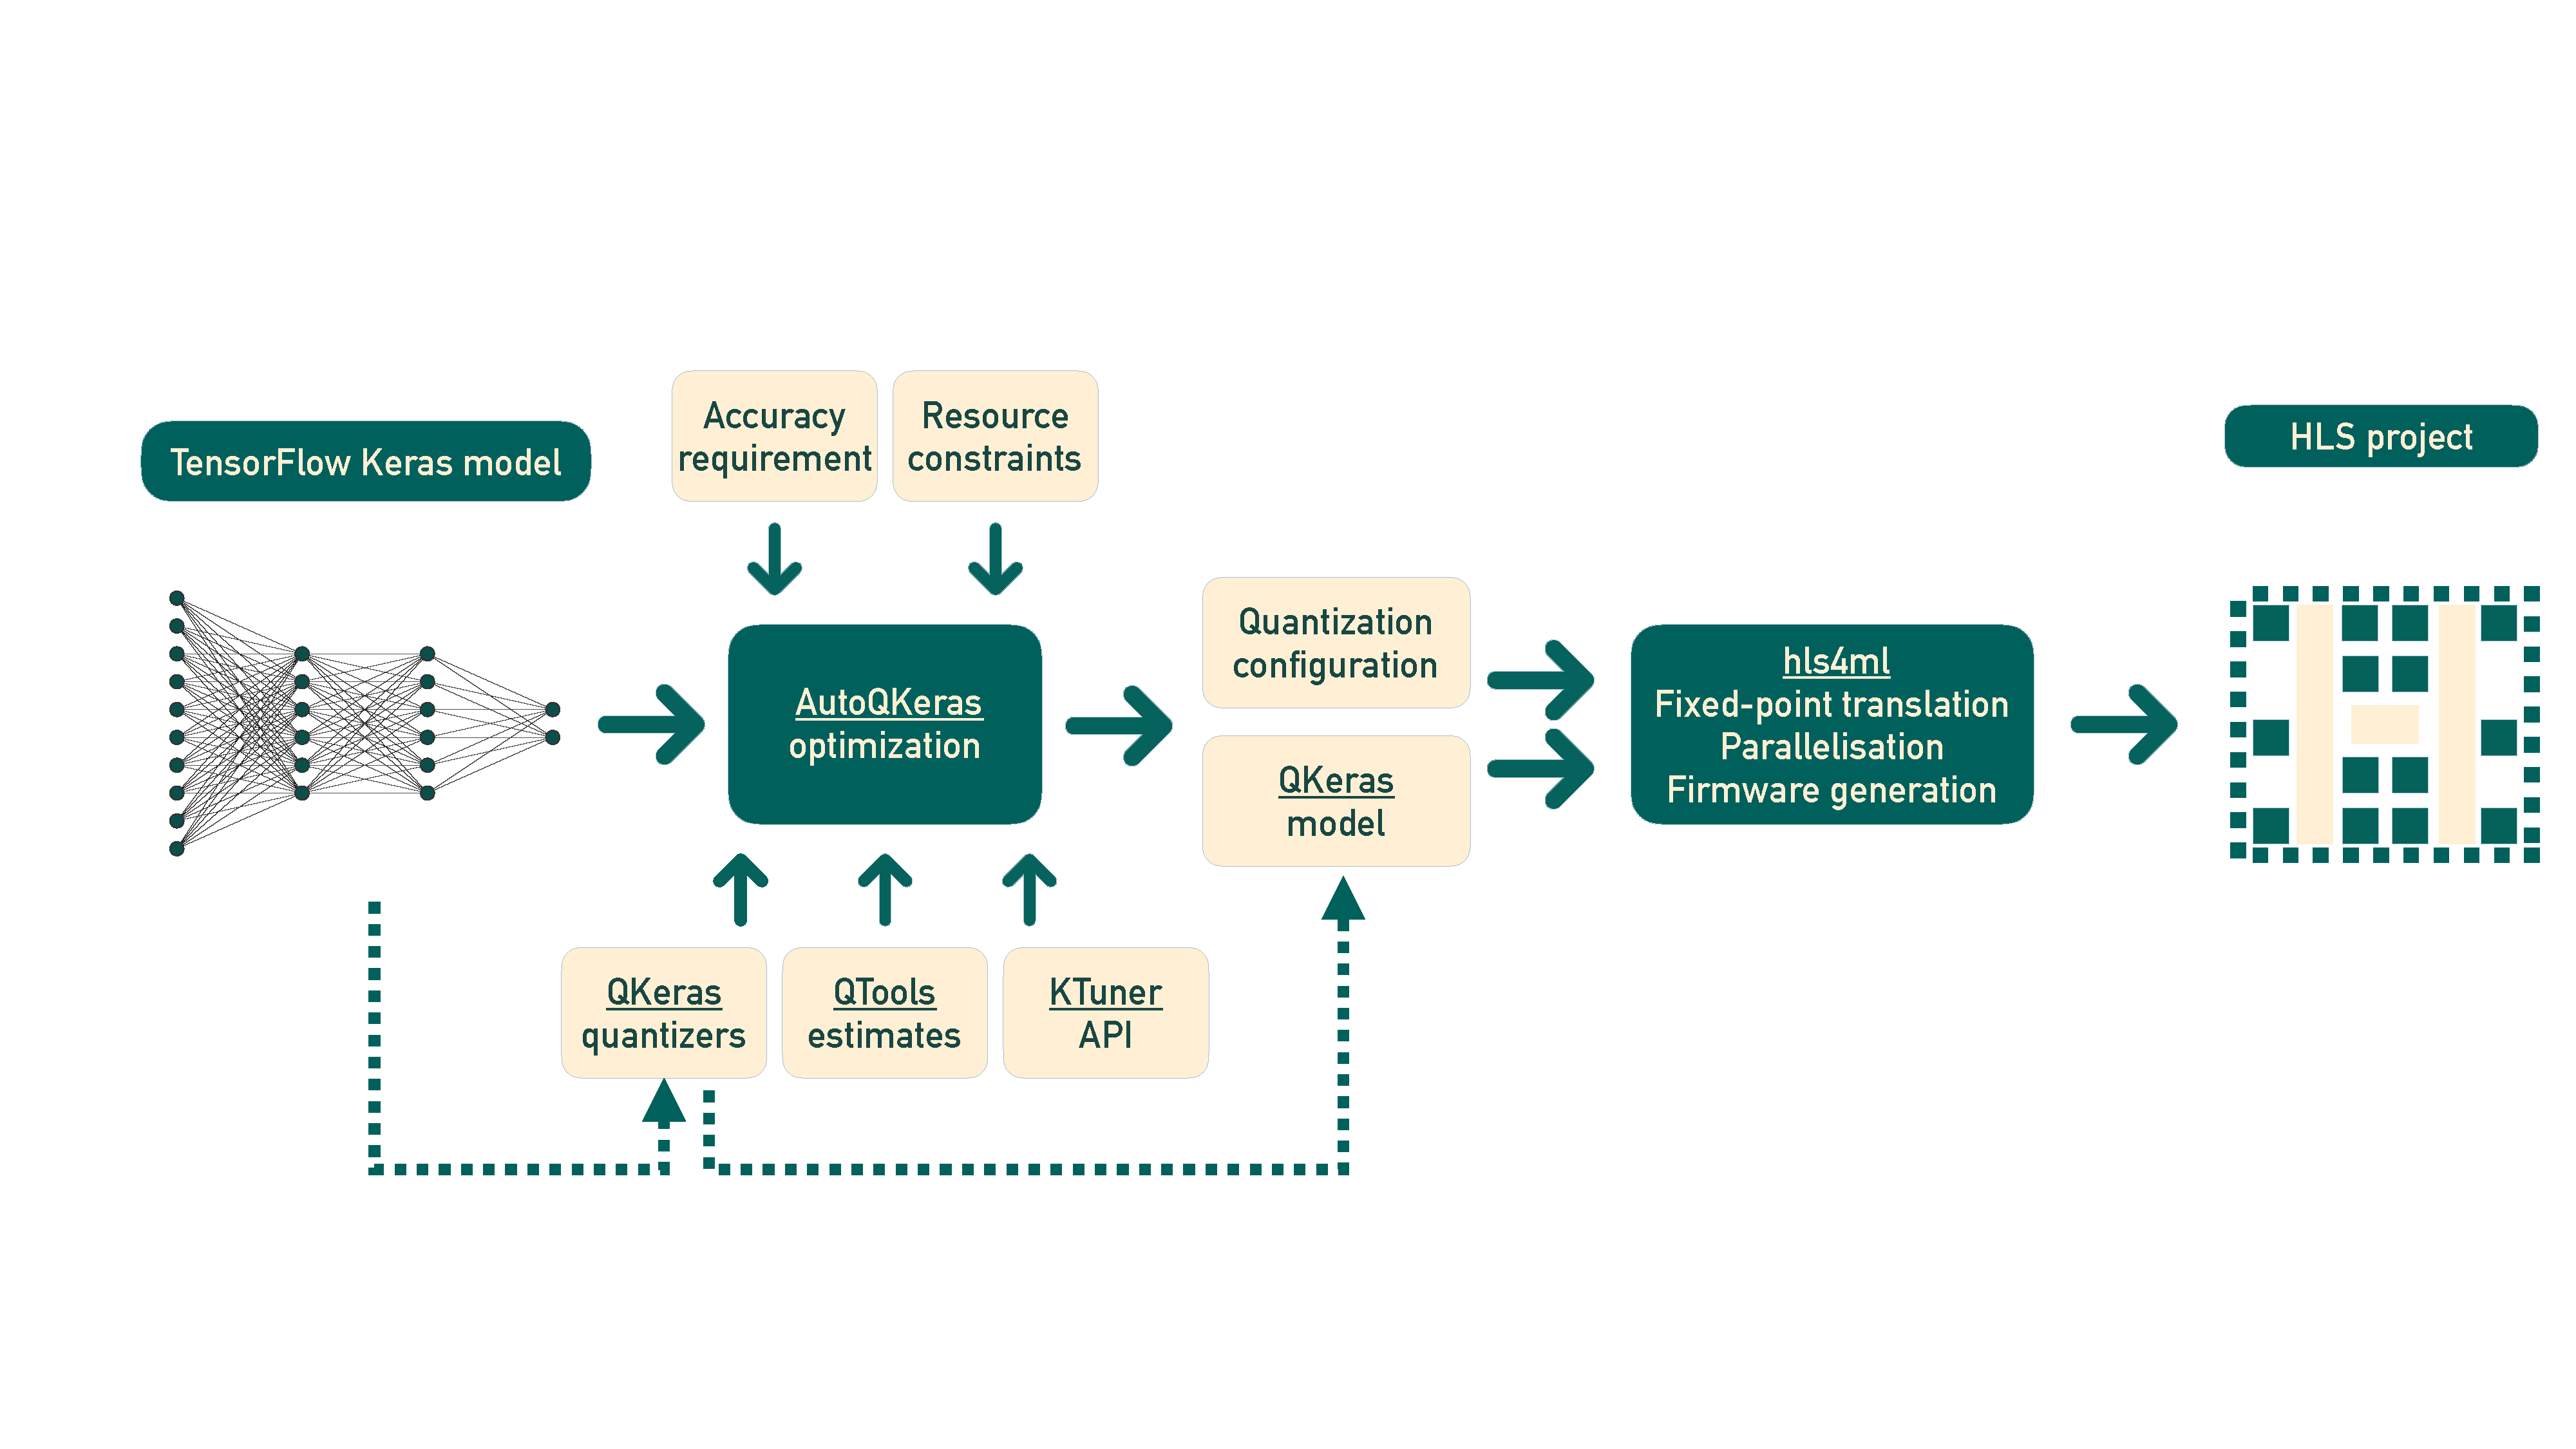
\includegraphics[width=0.99\textwidth]{figures/workflow.pdf}
%    \caption{The \hlsfml+QKeras workflow starts from a baseline TensorFlow Keras Model, which is converted into an optimally heterogeneously quantized equivalent, and then translated into highly parallel firmware~\cite{Coelho:2020zfu}.}
%    \label{figs2:workflow}
%\end{figure}
%Starting from a TensorFlow Keras model, the user can perform a hyperparameter scan over the type of quantization to be used per layer and parameter type usin AutoQKeras (an integral part of the QKeras package). Simultaneously, a scan is performed over the optimal number of filters (for convolutional layers) or neurons (for dense layers) for a given quantized model, as this is expected to change when quantizing a layer aggressively. User-specified parameters like the desired reduction in model energy, or model size, and the tolerated drop in model accuracy, can be passed as constraints in the search. An AutoML-type scan which considers both accuracy and model energy consumption (or size in bits) is then performed using the KerasTuner~\cite{kerastuner} framework as a back-end. The result is a hardware-aware Bayesian Optimization over a list of permitted quantizations and number of filters/neurons per layer. The resulting QKeras model is then translated into FPGA firmware using \hlsfml, which handles the translation into fixed point equivalents of the QKeras quantized weights and activations. As demonstrated in~\cite{aarrestad2021fast}, these quantized models can be pruned with no additional overhead using the TensorFlow Pruning API~\cite{zhu2017prune}.
The \hlsfml library currently provides support for several commonly used neural network layers like fully connected, convolutional, batch normalization, pooling, as well as several activation functions.
%Recently, support for large convolutional layers has also been added~\cite{aarrestad2021fast}.
These implementations are already sufficient to provide support for the most common architectures envisioned for deployment at L1.
%The workflow has been tested and validated both for DNNs~\cite{Coelho:2020zfu} and CNNs~\cite{aarrestad2021fast}. An example is shown in Figure~\ref{fig:accuracy_all} for a CNN tested on the Street View House Numbers (SVHN) Dataset~\cite{Netzer2011}. Here, the model accuracy (left) and DSP consumption (right) is scanned as a function of bit width for models which have been trained quantization-aware with QKeras (Q), additionally pruned with TensorFlow Pruning (QP) and models which have been quantized post training (BF and BF). The performance of these are compared to a model obtained using AutoQKeras automatic quantization tool (AQ) and its pruned equivalent (AQP). Using QKeras quantization-aware training, high accuracy can be maintained down to very narrow bit-widths, while significantly reducing the FPGA resource-consumption. 
%\begin{figure}[hbt]
%    \centering
%    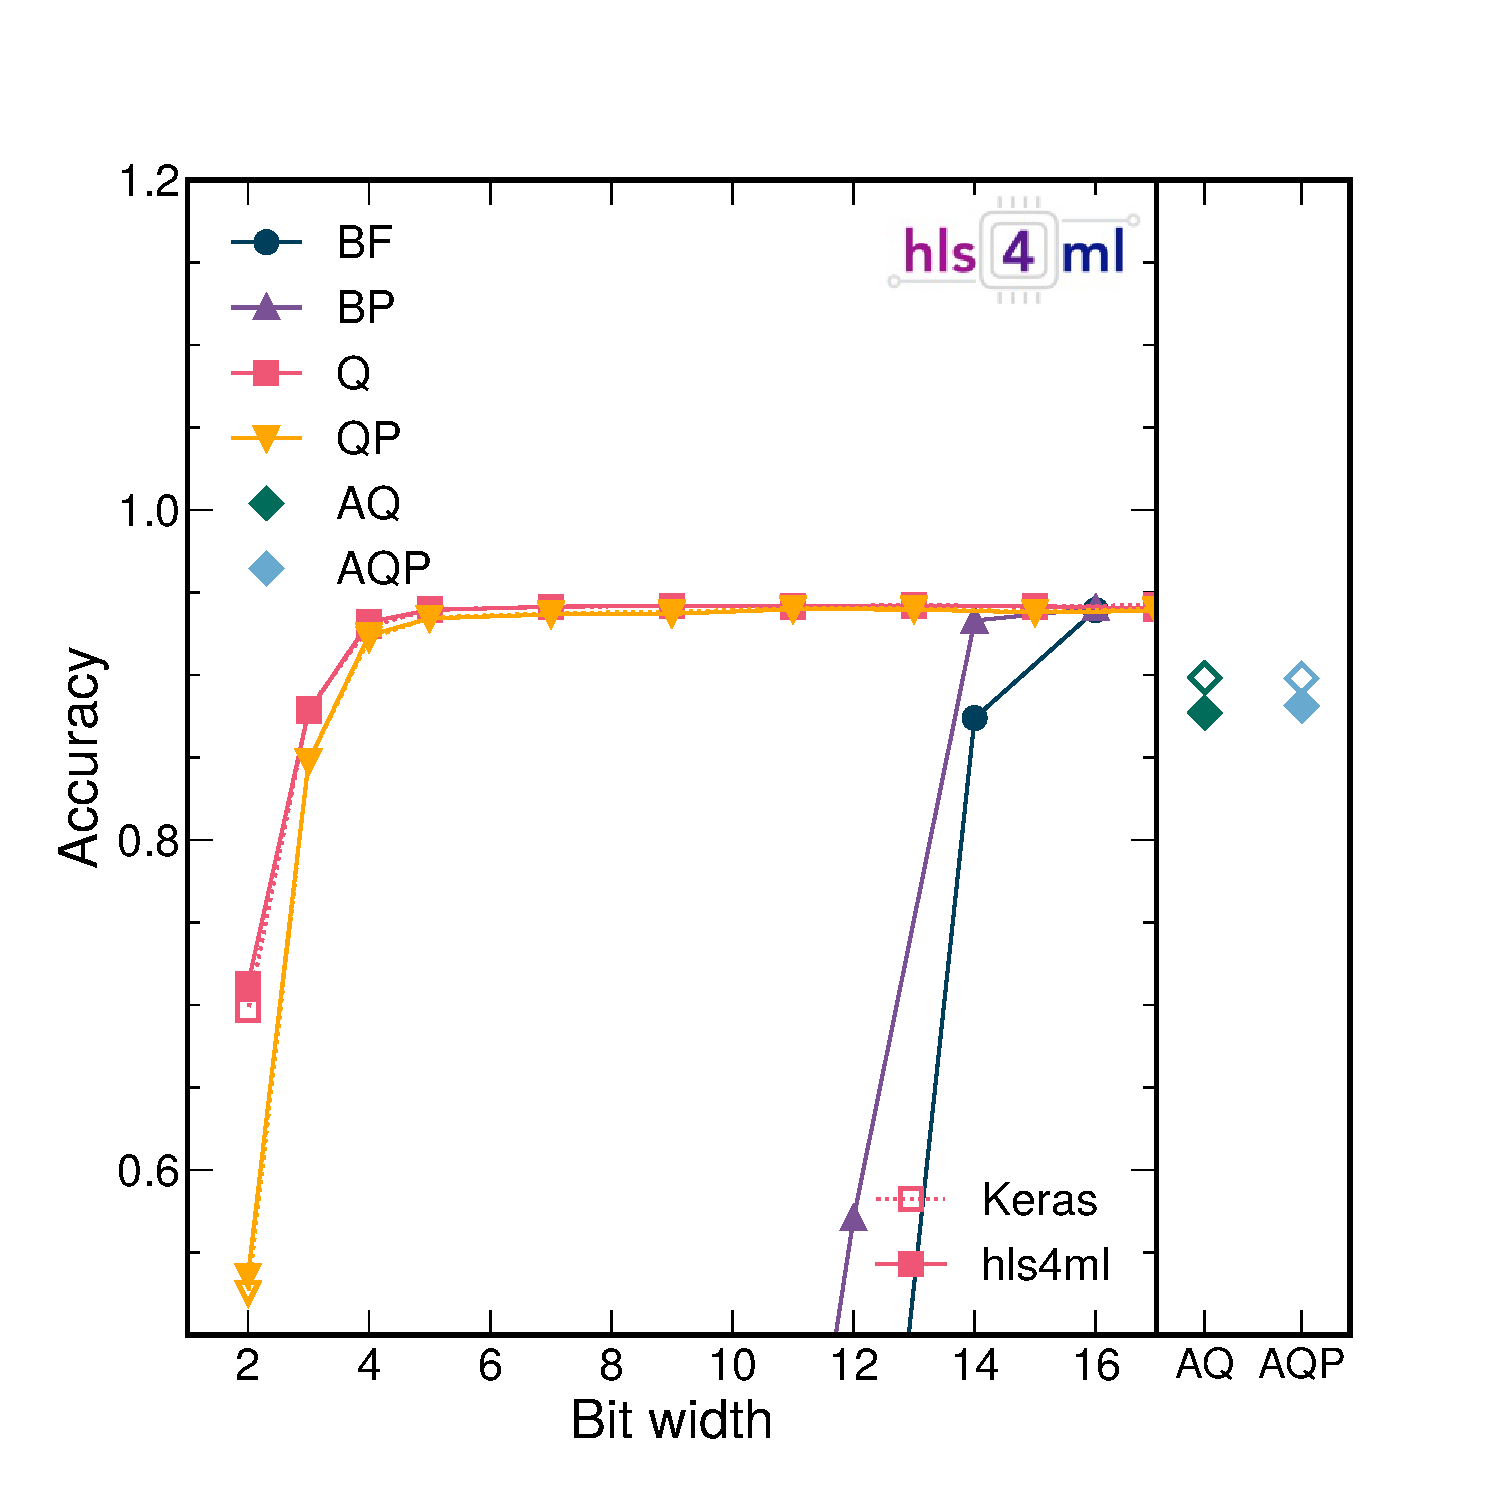
\includegraphics[width=0.45\textwidth]{figures/perModel_wAQ_scan_accuracy.pdf}
%    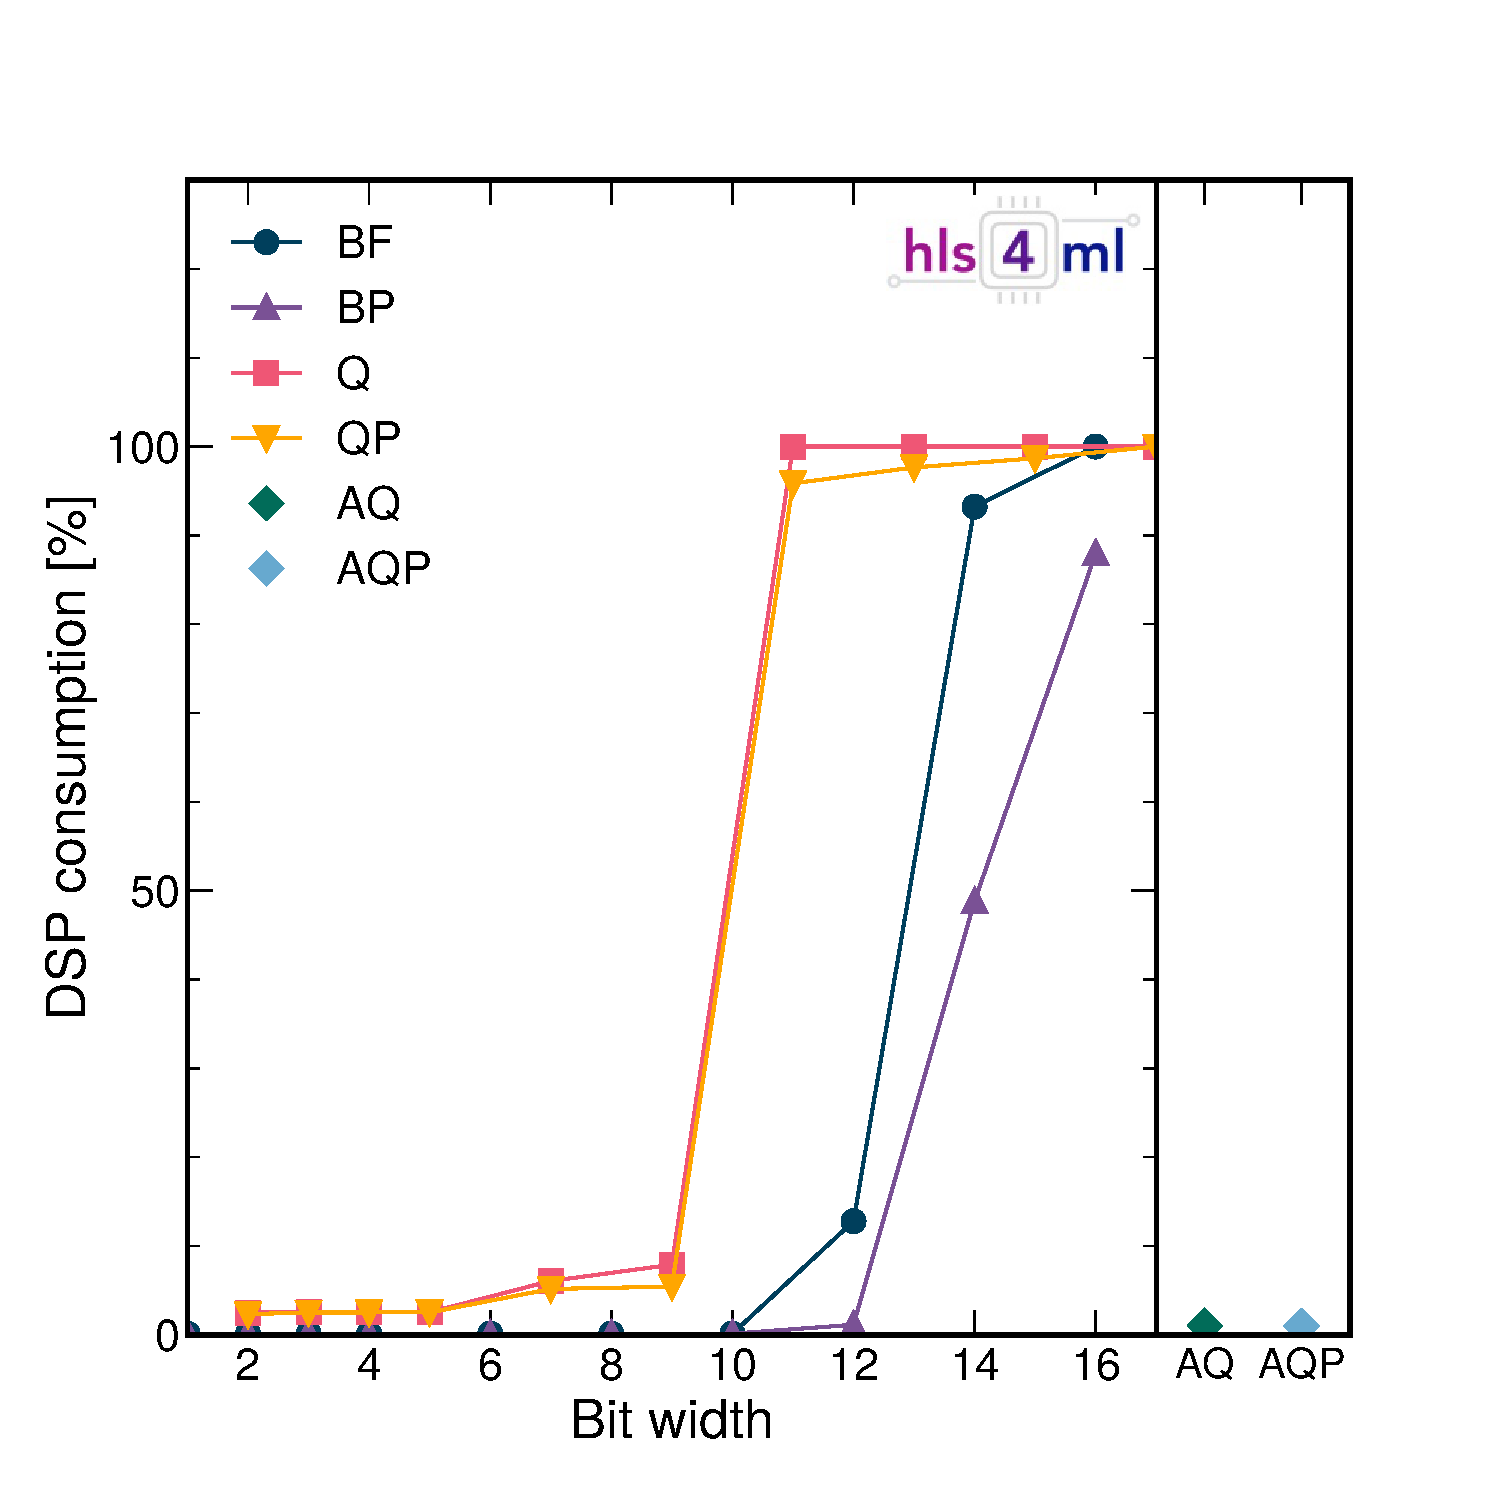
\includegraphics[width=0.45\textwidth]{figures/perModel_wAQ_scan_dsp.pdf}
%    \caption{Left: Model accuracy as a function of bit width for the Baseline Floating-point (BF), Baseline Pruned (BP), QKeras (Q) and QKeras Pruned (QP) models. 
%    The heterogeneously quantized models AutoQ (AQ) and AutoQ Pruned (AQP) are shown in the sidebar. Right}
%    \label{fig:accuracy_all}
%\end{figure}
%For extremely resource-constrained applications, \hlsfml offers support for binary or ternary networks~\cite{DiGuglielmo:2020eqx}. The typically achievable latency is of ${\cal O}(100)~$ns for DNNs and ${\cal O}(1)~\mu$s for CNNs.

%Examples of DNNs designed for the Level-1 trigger, include algorithms for the identification of VBF Higgs boson production events, as presented in Section 4.3.6 of Ref~\cite{CERN-LHCC-2020-004}. Specifically, the challenging final states where the Higgs decays into a pair of neutrinos or a pair of bottom quarks are targeted. Traditionally, cut-based selection algorithms have been used for these purposes, in order to stay within the imposed latency- and resource-budget. However, with the arrival of tools like \hlsfml and QKeras, ML alternatives are being explored.
% Figure~\ref{fig:VBFH_NN} shows the increase in signal acceptance that would be possible if replacing the current cut-based trigger algorithms by DNNs for VBF H$\rightarrow \nu \nu$ (left) and VBF H$\rightarrow b \bar{b}$ (left) processes. An increase in signal efficiency for VBF H$\rightarrow b \bar{b}$ (VBF H$\rightarrow \nu \nu$) of 36\% (15\%) with respect to the efficiency one would obtain using the logical OR of all the relevant cut-based triggers is observed. 
% \begin{figure}[hbt]
%     \centering
%     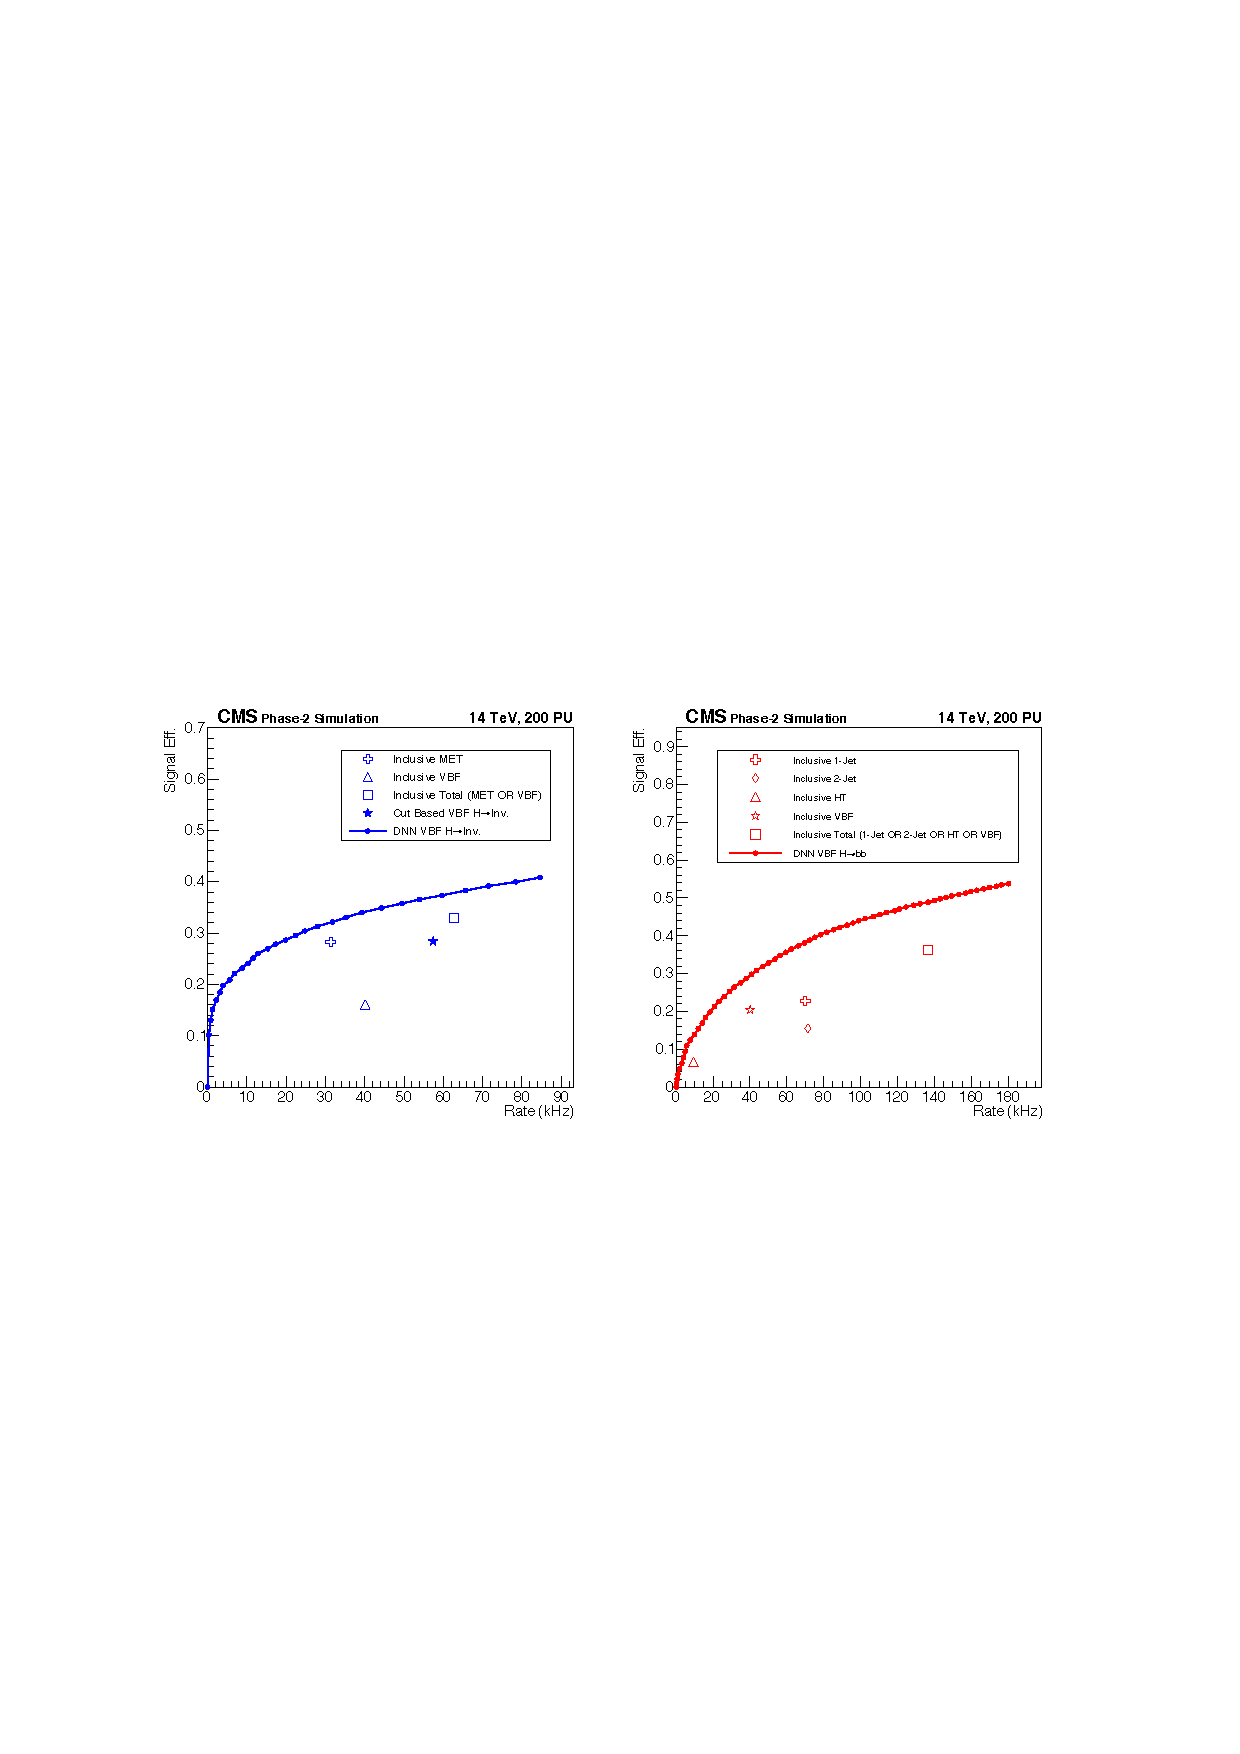
\includegraphics[width=0.95\textwidth]{figures/VBFH_NN.pdf}
%     \caption{Level-1 trigger efficiency versus rate for VBF H$\rightarrow \nu \nu$ (left) and VBF H$\rightarrow b \bar{b}$ (right) processes. The markers represent various cut-based algorithms and the solid lines corresponds to dedicated VBF DNNs~\cite{CERN-LHCC-2020-004}.}
%     \label{fig:VBFH_NN}
% \end{figure}
%When using \hlsfml to deploy these on hardware, a similar latency to that of cut-based trigger algorithms has been achieved (corresponding to a total latency of 9 bunch crossings).
First examples of machine learning models designed for the L1 trigger are based on fully connected layers and proposed for several physics tasks including the reconstruction and calibration of final physics objects as well as of lower level inputs such that trajectories, vertices, and calorimeter clusters~\cite{CERN-LHCC-2020-004}. Another application includes the identification of highly interesting and challenging events such as the ones with Higgs bosons produced through vector boson fusion and decaying into a pair of neutrinos or a pair of bottom quarks. 
One example of a convolutional NN architecture targeting the L1 trigger, is a dedicated algorithm for the identification of long-lived particles~\cite{Alimena_2020}. Here, an attempt is made to efficiently identify showers from displaced particles in a high granularity forward calorimeter. The algorithm is demonstrated to be highly efficient down to low energies while operating at a low trigger rate.
Traditionally, cut-based selection algorithms have been used for these purposes, in order to meet the limited latency- and resource-budget. However, with the advent of tools like \hlsfml and QKeras, ML alternatives are being explored to improve the sensitivity to such physics processes while maintaining latency and resources in the available budget.

%Other examples include variational auto-encoders~(VAE) for anomaly detection, as described in Section 3.7.2.1 of Ref.~\cite{CERN-LHCC-2020-004} and in Ref.~\cite{vaemining}.
%Here, a variational auto-encoder is  designed to correctly identify and trigger on non-Standard Model like events, with the ultimate goal of providing a stream of highly anomalous events. The algorithm is designed to run in the Level-1 Global Trigger, using as input a subset of particles fed into the system, like missing transverse energy and four-vectors of the five highest-$p_{T}$ jets. Jets are then classified as anomalous by the algorithm based on some cut on the degree of anomaly, ultimately decided upon based on the available bandwidth.

More recently, (variational) auto-encoders (VAEs or AEs) are being considered for the detection of "anomalous" collision events, i.e. events that are not produced by standard physics processes but that could be due instead to new unexpected processes never explored so far at colliders. Such algorithms have been proposed for both the incoming LHC run starting in 2022 as well as for the future high-luminosity runs where more granular information will be available. The common approach uses global information about the event, including a subset of individual produced particles or final physics objects such as jets as well as energy sums. The algorithm trained on these inputs is then used to classify the event as anomalous if surpassing a threshold on the degree of anomaly (typically the loss function), ultimately decided upon the available bandwidth.
%Currently, work is ongoing to improve and to deploy these anomaly detection algorithms in the CMS hardware triggering system for Run 3. Two possibilities are simultaneously being explored: Deployment in the Level-1 hardware trigger, and deployment in a dedicated {\em 40 MHz scouting system}.
%Scouting at 40 MHz consists of acquiring the L1 trigger data at the full bunch crossing rate of 40 MHz and analyzing certain interesting topologies at the full rate~\cite{CERN-LHCC-2020-004}. A proof-of-principle system, connected directly to the L1 trigger through 25 GB/s optical links and fed to a buffering/analysis system consisting of FPGAs and GPUs, has been successfully tested using inputs from the CMS Global Muon Trigger. This system would provide an excellent platform to test online anomaly detection algorithms before integration in the hardware trigger, and could also be used to run anomaly detection at a higher rate than what would be possible in the Global Trigger. 
Deploying a typical variational autoencoder is impossible in the L1-trigger since the bottleneck layer involves Gaussian random sampling. The explored solution is therefore to only deploy the encoder part of the network, and do inference directly from the latent dimension. Another possibility is to deploy a simple auto-encoder with the same architecture and do inference computing the difference between output and input. However, this would require to buffer a copy of the input for the duration it takes the auto-encoder to process the input.
For this reason, the two methods are being considered and compared in terms of accuracy over a range of new physics processes, as well as latency and resources.
%The two methods will be compared in terms of accuracy, latency and resource-consumption. Two possible architectures are currently being investigated: fully-connected and convolutional. Benchmarking is performed on a dataset simulated using the \texttt{DELPHES3} software~\cite{deFavereau:2013fsa} to emulate the CMS detector effects, but the model will eventually be trained on minimum bias data. A wide range of beyond standard model signal samples are used for comparing the performance of different models, and the one which performs the best on average for the different signal hypotheses, will be deployed in the CMS Level-1 trigger in Run 3.

%With the \hlsfml+QKeras workflow and the TensorFlow Pruning API, the goal is to be able to cater for all the different FPGA- and ASIC- based experiments at LHC (and other areas which require ultra low latency inference).
%However, some problems require more complicated architectures and NN layers. Specific layers can therefore easily be added to the \hlsfml library.
Finally, another interesting aspect of the \hlsfml tool is the capability for users to easily add custom layers that might serves a specific task not captured by the most common layers supported in the library. One example of this is compressed distance-weighted graph networks~\cite{garnet}, where a graph network block called a {\em GarNet layer}, takes as input a set of V vertices, each of which has $F_{in}$ features, and returns the same set of vertices with $F_{out}$ features. To keep the dimensionality of the problem at a manageable level, the input features of each vertex are encoded and aggregated at $S$ aggregators. Message-passing is only performed between vertices and a limited set of aggregators, and not between all vertices, significantly reducing the network size. In Ref.~\cite{garnet}, an example task of pion and electron identification and energy regression in a 3D calorimeter is studied. A total inference latency of ${\cal O}(100)~$ns is reported, satisfying the L1 requirement of ${\cal O}(1)~\mu$s latency. The critical resource is Digital Signal Processing (DSP) units, where 29\% of the DSPs are in use by the algorithm. This can be further reduced by taking advantage of quantization-aware training with QKeras. Another example of a graph neural network architecture implemented on FPGA hardware using \hlsfml, is presented in Ref.~\cite{heintz2020accelerated}. This work shows that a compressed GNN can deployed on FPGA hardware within the latency and resources required by L1 trigger system for the challenging task of reconstructing the trajectory of charged particles.
%This GNN is designed to identify the trajectory of charged particles, an extremely challenging task where current algorithms scale worse than quadratically in the number of hits. Even for this complicated task, a latency of ${\cal O}(1)~\mu$s can be achieved for a compressed GNN architecture. The algorithm is described in detail in Section~\ref{sec:lhceventreco} above.
Thes are important results as demonstrating that more advanced and custom neural network architectures can be successfully deployed in the Level-1 trigger system. 

In many cases, the task to be performed is simple enough that a Boosted Decision Tree (BDT) architecture suffices to solve the problem. As of today, BDTs are still the most commonly used ML algorithm for LHC experiments. To simplify the deployment of these, the library {\tt Conifer}~\cite{Summers:2020xiy} has been developed. In {\tt Conifer}, the BDT implementation targets extreme low latency inference by executing all trees, and all decisions within each tree, in parallel. BDTs and RandomForests can be converted from scikit-learn~\cite{scikit-learn}, XGBoost~\cite{XGBoost}, and TMVA~\cite{TMVA}, with support for more BDT training libraries planned.

There are several ongoing projects at LHC which plan to deploy BDTs in the Level-1 trigger using {\tt Conifer}. One example is a BDT designed to provide an estimate of the {\em track quality}, by learning to identify tracks which have been reconstructed due to error in the reconstruction process, and do not originating from a real particle~\cite{bdt_tq}. Both DNN and BDT architectures are explored.
%Both a DNN and BDT architecture is explored and the results are shown in Figure~\ref{figs2:bdt_tq}.
%\begin{figure}[hbt]
%    \centering
%    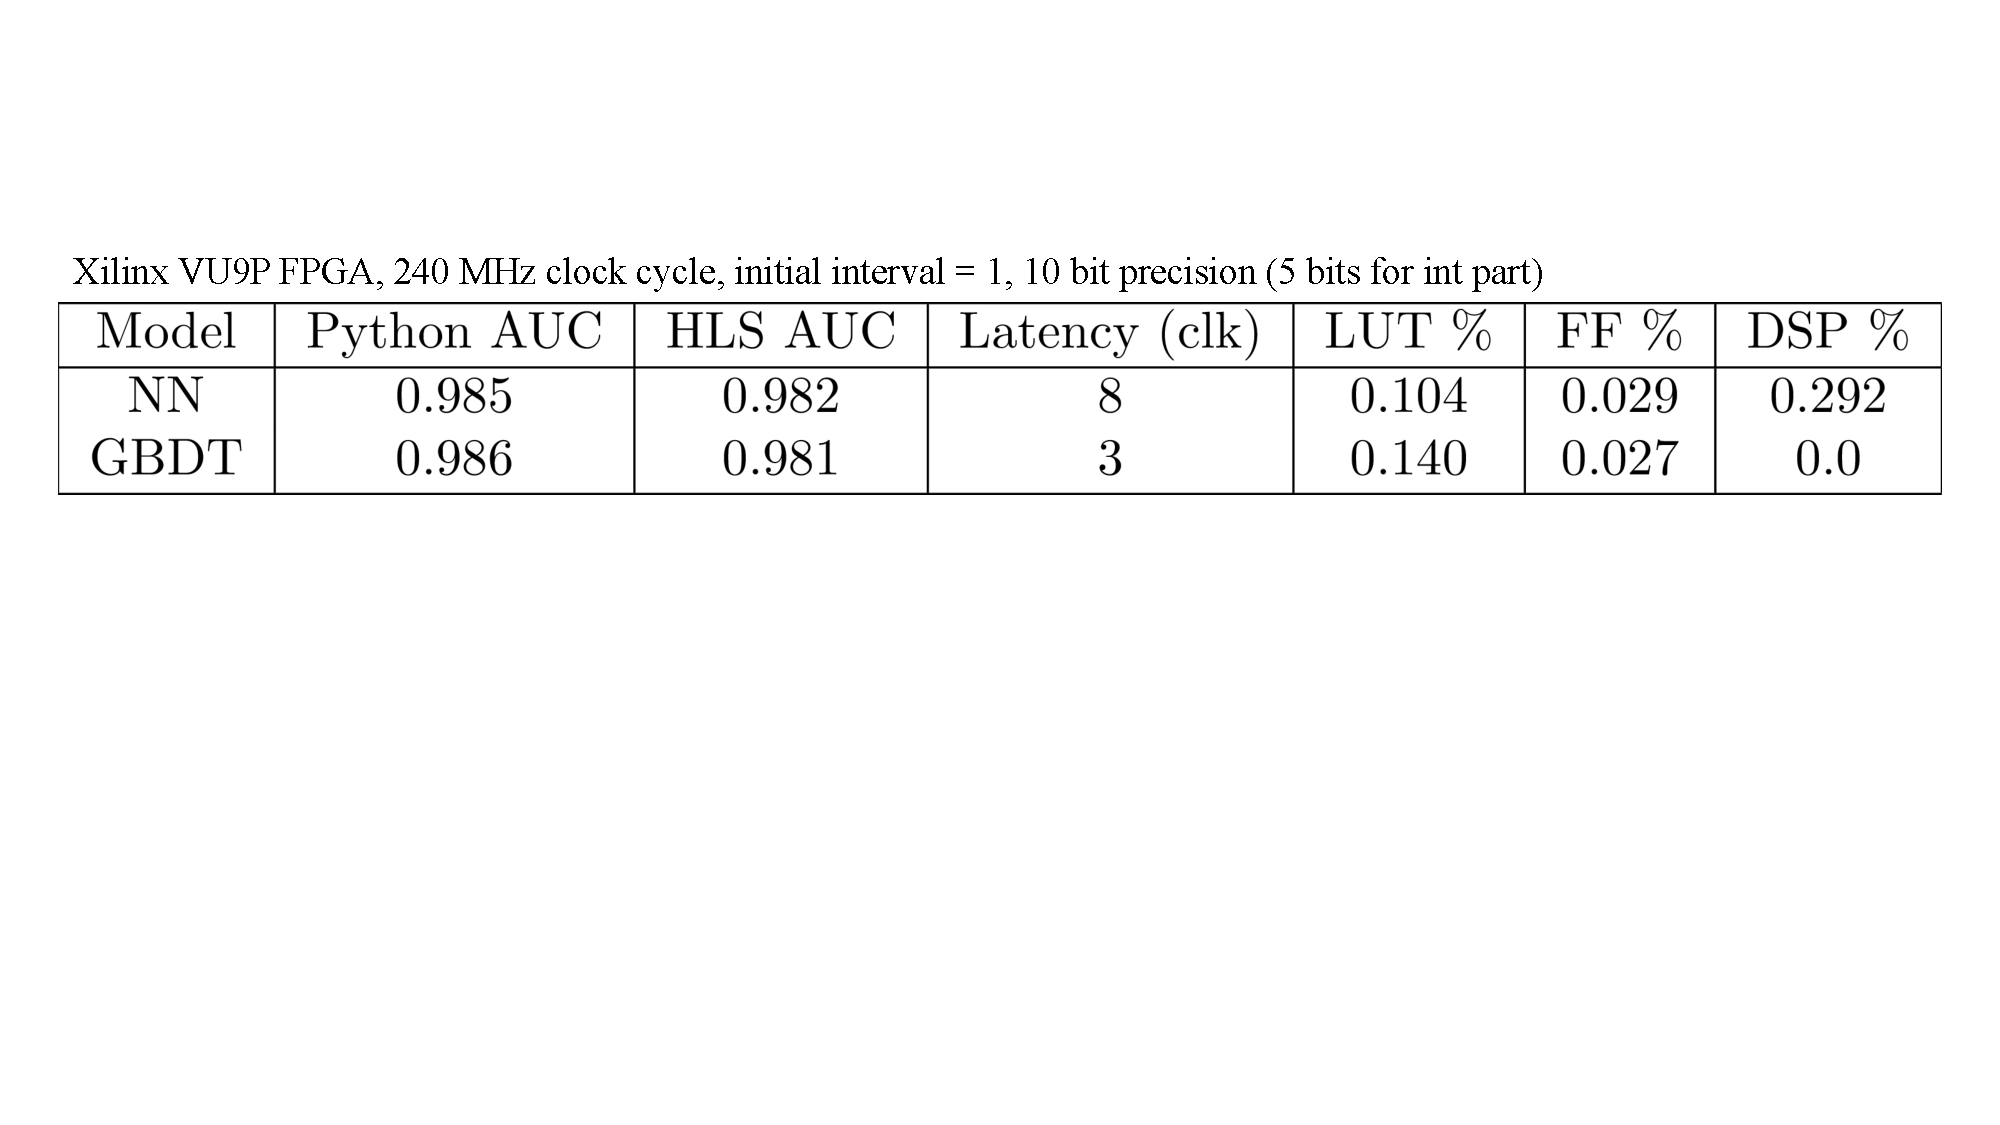
\includegraphics[width=0.70\textwidth]{figures/bdt_trackquality.pdf}
%    \caption{Accuracy, latency and resource usage for a track quality algorithm using a BDT or a DNN %architecture~\cite{bdt_tq}.}
%    \label{figs2:bdt_tq}
%\end{figure}
While the accuracy and resource-usage are similar, the latency is significantly reduced for a BDT architecture. The algorithm is planned to be implemented in the CMS Experiment for the Phase 2 data taking period at LHC.
%Another example is a BDT for electron and photon identification for the CMS High Granularity Endcap Calorimeter, described in Section 3.2.3 of Ref.~\cite{CERN-LHCC-2020-004}. Signal candidates are distinguished from clusters originating from pileup using five longitudinal and four lateral shower shape variables.

While the \hlsfml library is based on High-Level Synthesis tools from FPGA vendors, other approaches are being considered based on a hardware description language such as VHDL~\cite{Nottbeck:2019rqu,Fritzsche2020}. One example is the application of ML for the real-time signal processing of the ATLAS Liquid Argon calorimeter~\cite{atlas1996atlas}. It has been shown that with upgraded capabilities for the HL-LHC collision environment the conventional signal processing, which applies an optimal filtering algorithm~\cite{Cleland:2002rya}, will lose its performance due to the increase of overlapping signals. More sophisticated DL methods have been found to be more suitable to cope with these challenges being able to maintain high signal detection efficiency and energy reconstruction. More specifically, studies based on simulation~\cite{madysa-chep} of dilated convolutional neural networks showed promising results. An implementation of this architecture for FPGA is designed using VHDL~\cite{Fritzsche2020} to meet the strict requirements on latency and resources required by the L1 trigger system. The firmware runs with a multiple of the bunch crossing frequency to reuse hardware resources by implementing time division multiplexing while using pipeline stages, the maximum frequency can be increased. Furthermore, DSPs are chained up to perform the MAC operation in between two layers efficiently. In this way, a core frequency of more than 480 MHz could be reached, corresponding to twelve times the bunch crossing frequency.

\subsubsection{Bringing ML to detector front-end}

While LHC detectors grow in complexity to meet the challenging conditions of higher-luminosity environments, growing data rates prohibit transmission of full event images off-detector for analysis by conventional FPGA-based trigger systems.
As a consequence, event data must be compressed on-detector in low-power, radiation-hard application specific integrated circuits (ASICs) while sacrificing minimal physics information.

Traditionally this has been accomplished by simple algorithms, such as grouping nearby sensors together, so that only these summed ``super-cells'' are transmitted, sacrificing the fine segmentation of the detector.
Recently, an autoencoder-based approach has been proposed, relying instead on a set of machine-learned radiation patterns to more efficiently encode the complete calorimeter image via a convolutional NN (CNN).
Targeting the High-Granularity Endcap Calorimeter (HGCal)~\cite{collaboration:2017gbu} at the HL-LHC, the algorithm aims to achieve higher-fidelity electromagnetic and hadronic showers, critical for accurate particle identification.

The on-detector environment (the ECON-T concentrator ASIC~\cite{collaboration:2017gbu}) demands a highly-efficient CNN implementation; a compact design should be thoroughly optimized for limited-precision calculations via quantization-aware training tools~\cite{qkeraspaper}.
Further, to automate the design, optimization, and validation of the complex NN circuit, HLS-based tool flows~\cite{Duarte:2018ite} may be adapted to target the ASIC form factor.
Finally, as the front-end ASIC cannot be completely reprogrammed in the manner of an FPGA, a mature NN design is required from the time of initial fabrication.
However, adaptability to changing run conditions and experimental priorities over the lifetime of the experiment motivate the implementation of all NN weights as configurable registers accessible via the chip's slow-control interface.

\subsection{High intensity accelerator experiments}
\subsubsection{Belle-II}
The Belle II experiment in Japan is engaged in the search for physics phenomena that cannot be explained by the Standard Model. Electrons and positrons are accelerated at the SuperKEKB particle accelerator to collide at the interaction point inside of the Belle II detector. The resulting decay products are continually measured online by the detector’s heterogenous sensor composition. Resulting data is then stored offline for detailed analysis. Due to the increasing luminosity (target luminosity is $8\times10^{35}\mathrm{cm}^{-2}\mathrm{s}^{-1}$) most of the recorded data is not a result from the electron positron annihilation experiment, coming from the interaction point, rather it is due to unwanted but unavoidable background reactions. Not only is storing all the data now inefficient due to the background rates from outside of the interaction point, but it is also often not even feasible to build the resulting infrastructure that stores all the generated data.  A multilevel trigger system is used as a solution to decide online which recorded events are to be stored. The Neural Network z-Vertex Trigger (NNT) described here is in a deadtime-free level 1 (L1) trigger and identifies particles by estimating their origin along the beampipe. For the whole L1 trigger process, from data readout to the decision, a real-time 5~\si{\micro\second} time budget is given to avoid dead-time \cite{Lai_2020}. Due to the data pre-processing and transmission, the NNT needs to provide a decision within 300 ns processing time.

The task of the NNT is to estimate the origin of a particle track, so that it can be decided whether it originates from the interaction point or not. For this purpose, a multilayer perceptron (MLP) implemented on a Xilinx Virtex 6 XC6VHX380T FPGA is used. The MLP consists of three layers with 27 input neurons, 81 hidden layer neurons and two output neurons. Data from the Belle II's Central Drift Camber (CDC) is used for this task, since it is dedicated to the detection of particle tracks. Before being processed by the network, the raw detector data is first combined into a 2D track based on so-called track segments, which are groupings of adjacent active sense wires. For the processing, five different networks are used, which are trained to compensate missing sensor data. The sense wires of the CDC are grouped in nine so called Super Layer (SL) which are divided into alternating axial and stereo layers. Since not all SLs are always providing data to be used for the estimation, the NNT selects an appropriate network online to compensate this. As output the NNT delivers the origin of the track in z, along the beampipe, as well as the polar angle $\theta$. With the help of the z-vertex, the downstream Global Decision Logic (GDL) can decide whether a track is from the interaction point or not. In addition, the particle momentum can be detected using the polar angle $\theta$ \cite{baehr2019low}. 

The networks used in the NNT are trained offline. The first networks were trained with plain simulated data because no experimental data was available. For newer networks, reconstructed tracks from the experimental data are used. For the training the iRPROP algorithm is used which is an extension of the RPROP backpropagation algorithm.

Current results show a good correlation between the NNT tracks and reconstructed tracks. Since the event rate and the background noise are currently still tolerable, the z-cut, i.e., the allowed estimated origin of a track origin in order to be kept, is chosen at +/- 40 cm. With increasing luminosity and the associated increasing background, this z-cut can be tightened.

Since the new Virtex Ultrascale based Universal Trigger Board (UT4) is available for the NNT this year, an extension of the data preprocessing is planned. This will be done by a 3D Hough transformation for further efficiency increases. It has already been shown in simulation that a more accurate resolution and larger solid angle coverage can be achieved \cite{Skambraks_2020}.

\subsubsection{Mu2e}
The Mu2e experiment at Fermilab will search for the charged lepton flavor violating process of neutrino-less $\mu \to e$ coherent conversion in the field of an aluminum nucleus. About $7\cdot 10^{17}$ muons, provided by a dedicated muon beam line in construction at Fermilab, will be stopped in 3 years in the aluminum target. The corresponding single event sensitivity will be $2.5\cdot 10^{-17}$. To detect the signal $e^-$ ($p=105$ MeV/c), Mu2e uses a detector system made of a straw-tube tracker and a crystal electromagnetic calorimeter~\cite{MU2E}. 

The trigger system is based on detector Read Out Controllers (ROCs) which stream out continuously the data, zero-suppressed, to the Data Transfer Controller units (DTCs). The proton pulses are delivered at a rate of about 600 kHz and a duty cycle of about 30\% (0.4 s out of 1.4 s of the booster-ring delivery period). Each proton pulse is considered a single event, with the data from each event then grouped at a single server using a 10 GBytes/second Ethernet switch. Then, the online reconstruction of the events starts and makes a trigger decision.  The trigger system needs to satisfy the following requirements: (1)  provide efficiency better than 90\% for the signals; (2)  keep the trigger rate below a few kHz -- equivalent to 7 Pb/year; (3) achieve a processing time $<5$~ms/event. Our main physics triggers use the information of the reconstructed tracks to make the final decision.  The current strategy is to perform the helix pattern-recognition and the track reconstruction with the CPUs of the DAQ servers, but so far this design showed limitations in matching the required timing performance~\cite{pezzullo_gianantonio_2020_4088480}. Another idea that the collaboration started exploring is to perform the early stage of the track reconstruction on the ROC and DTC FPGA using the High Level Synthesis tool (HLS) and the \texttt{hls4ml} package. The Mu2e helix pattern-recognition algorithms~\cite{pezzullo_gianantonio_2020_4088480} are a natural fit for these tools for several reasons: they use neural-networks to clean up the recorded straw-hits from hits by low-momentum electrons ($p<10$~MeV/c) and they perform large combinatorics calculations when reconstructing the helicoidal electron trajectory. This R\&D is particularly important for the design of the trigger system of the planned upgrade of Mu2e~\cite{abusalma2018expression}, where we expect to: (i) increase the beam intensity by at least a factor of 10, (ii) increase the duty cycle to at least 90\%, and (iii) increase the number of detector's channels to cope with the increased occupancy.


\subsection{Materials Discovery}
\subsubsection{Materials Synthesis}

\paragraph*{\textbf{Context}} Advances in electronics, transportation, healthcare, and buildings require the synthesis of materials with controlled synthesis-structure-property relationships. To achieve application-specific performance metrics, it is common to design and engineer materials with highly-ordered structures. This directive has led to a boom in non-equilibrium materials synthesis techniques. Most exciting are additive synthesis and manufacturing techniques, for example, 3d-printing\cite{Wang2020-tv,Parekh2016-vj,Visser2015-hy,Ligon2017-dg,Zarek2016-dw} and thin film deposition\cite{Chrisey1994-gw,Richter1990-ml,Yoshino2000-oo,Kelly2000-xk,Marvel2013-cd,George2010-pb,Park2001-so}, where complex nanoscale architectures of materials can be fabricated. To glean insight into synthesis dynamics, there has been a trend to include in situ diagnostics to observe synthesis dynamics\cite{Ojeda-G-P2017-la,Egelhoff1989-pr,Thomas1999-ij,Langereis2007-dj}. There is less emphasis  on automating the downstream analysis to turn data into actionable information that can detect anomalies in synthesis, guide experimentation, or enable closed-loop control. Part of the challenge with automating analysis pipelines for in situ diagnostics is the highly variable nature and multimodality of the measurements and the sensors. A system might measure many time-resolved state variables (time-series) at various locations (e.g., temperature, pressure, energy, flow rate, etc.)\cite{Hansen1999-an}. Additionally, it is common to measure time-resolved spectroscopic signals (spectrograms) that provide, for instance, information about the dynamics of the chemistry and energetic distributions of the materials being synthesized\cite{Cooks2018-jm,Termopoli2019-gb,Dauchot1995-cu,Aubriet2002-ln}. Furthermore, there are a growing number of techniques that leverage high-speed temporally-resolved imaging to observe synthesis dynamics\cite{Trigub2017-xw,Ojeda-G-P2018-cv}.

        
\paragraph*{\textbf{Challenges}}: Experimental synthesis tools and in situ diagnostic instrumentation are generally semi-custom instruments provided by commercial vendors. Many of these vendors rely on proprietary software to differentiate their products from their competition. In turn, the closed-nature of these tools and even data schemas makes it hard to utilize these tools fully. The varied nature and suppliers for sensors compounds this challenge. Integration and synchronization of multiple sensing modalities require a custom software solution. However, there is a catch-22 because the software does not yet exist. Researchers cannot be ensured that the development of analysis pipelines will contribute to their ultimate goal to discover new materials or synthesize materials with increased fecundity. Furthermore, there are significant workforce challenges as most curriculums emphasize Edisonian rather than computational methods in the design of synthesis. There is an urgent need for multilingual trainees fluent in typically disparate fields. 

        
\paragraph*{\textbf{Existing and Planned Work}}:Recently, the materials science community has started to embrace machine learning to accelerate scientific discovery\cite{Butler2018-qo,Schmidt2019-dz,Ramprasad2017-wp}. However, there have been growing pains. The ability to create highly-overparameterized models to solve problems with limited data provides a false sense of efficacy without generalization required for science. Machine learning models architectures designed for natural time-series and images are ill-posed for physical processes governed by equations. In this regard, there is a growing body of work to embed physics in machine learning models, which serve as the ultimate regularizers. For instance, rotational\cite{Oxley2020-hg,Kalinin2020-xl} and Euclidian equivariance\cite{Smidt_undated-oh,Smidt2020-sh} has been built into the model architectures, and methods to learn sparse representations of underlying governing equations have been developed\cite{Kaheman2020-zt,De_Silva2020-ef,Champion2019-kh}. Another challenge is that real systems have system-specific discrepancies that need to be compensated\cite{Kaheman2019-yu}. For example, a precursor from a different batch might have as slightly different viscosity that needs to be considered.  There is an urgent need to develop these foundational methods for materials synthesis. Complementing these foundational studies, there has been a growing body of literature emphasizing post-mortem machine-learning-based analysis of in situ spectroscopies\cite{Provence2020-ro,Trejo2019-ph}. As these concepts become more mature, there will be an increasing emphasis on codesign of synthesis systems, machine learning methods, and hardware for on-the-fly analysis and control. This effort towards self-driving laboratories is already underway in wet-chemical synthesis where there are minimal dynamics, and thus, latencies are not a factor\cite{MacLeod2020-mv,Langner2020-ds}. Furture efforts will undoubtedly focus on controlling dynamic synthesis processes where ms-to-ns latencies are required.

\subsubsection{Scanning Probe Microscopy}
\begin{itemize}
    \item \textbf{Context:} Touch is the first sense humans develop. Since the atomic force microscope’s (AFM) invention in 1985\cite{Binnig1986-ig}, humans have been able to “feel” surfaces with atomic-level resolution with pN sensitivity. AFMs rely on bringing an atomically-sharp tip mounted on a cantilever into contact with a surface. By scanning this tip nanometer-to-atomically resolved images can be constructed by measuring the angular deflection of a laser bounced off the cantilever. This detection mechanism provides high-precision sub-angstrom measures of displacement. By adding functionality to the probe (e.g., electrical conductivity\cite{Benstetter2009-oe}, resistive heaters\cite{King2005-sc}, single-molecule probes\cite{Oberhauser2002-cs}, N-V centers\cite{Ariyaratne2018-hg}, etc.). Scanning probe microscopy (SPM) can measure of nanoscale functional properties, including electrical conductivity\cite{Seidel2010-uv,Gomez-Navarro2005-pu}, piezoresponse\cite{Jesse2011-tv}, electrochemical response\cite{Jesse2012-gh}, magnetic force\cite{Kazakova2019-dj}, magnetometry\cite{Casola2018-ms}, and much more. These techniques have been expanded to include dynamics measurements where measurements occur during a tip-induced perturbation that drives a structural transformation. These methods have led to a boom in new AFM techniques, including fast-force microscopy\cite{Benaglia2018-js}, current-voltage spectroscopies\cite{Holstad2020-kq}, band-excitation-based spectroscopies\cite{Jesse2018-jw}, and full-acquisition mode spectroscopies\cite{Somnath2015-qk}. What has emerged is a data deluge where these techniques are either underutilized or under-analyzed.
    \item \textbf{Experimental Challenges and Constraints:} The key practical challenges are that it takes on days-to-weeks to analyze data from a single measurement properly. As a result, experimentalists are caught unawares of how to design their experiments. There is even minimal feedback if the experiments are without artifacts (e.g., tip damage) that renders the experiments unusable. The number of costly failed experiments is a strong deterrent to conducting advanced scanning probe spectroscopies and developing even more sophisticated imaging techniques. There is a significant challenge in both the acceleration and automation of analysis pipelines. 
    \item \textbf{Existing Work and Opportunities:} In materials science, scanning probe microscopy has quickly adopted machine learning. Techniques for linear and nonlinear spectral unmixing provide rapid visualization and extraction of information from these datasets to discover and unravel physical mechanisms\cite{Ziatdinov2020-nt,Collins2020-na,Kalinin2021-gp,Collins2020-ml}. The ease of applying these techniques has led to justified concerns about the overinterpretation of results and overextension of linear models\cite{Griffin2020-mc} to highly nonlinear systems. More recently, long-short term memory autoencoders are controlled to have non-negative and sparse latent spaces for spectral unmixing. By traversing the learned latent space, it has been possible to draw complex structure-property relationships\cite{Agar2019-eq,Holstad2020-kq}. There are significant opportunities to accelerate computational pipeline such that information can be extracted on practically relevant time scales by the experimentalist on the microscope. Due to the high velocity of data, up to GB/s, with sample rates of 100,000 spectra extracting even cursory information will require the confluence of data-driven models, physics informed machine learning and AI hardware. As a tangible example, in band-excitation piezoresponse force microscopy, the frequency-dependent cantilever response is measured at rates up to 2,000 spectra-per-second. Extracting the parameters from these measurements requires fitting the response to an empirical model. Using least-squares fitting throughput is limited to ~50-fits/core-minute, neural networks provide an opportunity to accelerate analysis and better handle noisy data\cite{Borodinov2019-pn}. There is an opportunity to deploy neural networks on GPU or FPGA hardware accelerators to approximate and accelerate by orders-of-magnitude this pipeline.
    
\end{itemize}
  
 

\subsubsection{Electron Microscopy}
\subsubsection{X-ray Spectroscopy}
\subsection{Fermilab Accelerator Controls}
    \begin{itemize}
        \item \textbf{Context}: 
            The Fermi National Accelerator Laboratory (Fermilab) is dedicated to investigating matter, energy, space and time \cite{fermilab_about}. For over 50 years, Fermilab's primary tool for probing the most elementary nature of matter has been its vast accelerator complex. Spanning a number of miles of tunnels, the accelerator complex is actually multiple accelerators and beam transport lines each representing different accelerator techniques and eras of accelerator technologies. In its long history, Fermilab's accelerator complex has had to adapt to the mission, asking more of the accelerators than they were designed for and often for purposes they were never intended. This often resulted in layering new controls on top of existing antiquated hardware. Until recently, accelerator controls focused mainly on providing tools and data to the machine operators and experts for tuning and optimization. Having recognized the future inadequacies of the current control system and the promise of new technologies such as ML, the Fermilab accelerator control system will be largely overhauled in the coming years as part of the Accelerator Controls Operations Research Network (ACORN) project \cite{acorn_paper}. 
        \item \textbf{Challenges}: 
            The accelerator complex brings unique challenges for machine learning. Particle accelerators are immensely complicated machines, each consisting of many thousands or variable components and even larger data sources. Their large size and differing types, resolution, and frequency of data, means collecting and synchronizing data is difficult. Also, as one might imagine, control and regulation of beams  that travel at near light speeds is always a challenge. Maintaining and upgrading the accelerator complex controls is costly, for this reason much of the accelerator complex is a mixture of obsolete, new and cutting edge hardware. 
            % Particle accelerators are immensely complicated machines, each with thousands of variable components. 
            % Keeping older accelerators running with higher demand than was ever designed for. 
            % Re-purposing accelerators for tasks they were never designed for. Overlaying advanced control algorithms atop of now obsolete control infrastructure. 
            % New accelerators having very tight design specs, machine protection critical. \cite{7454846}
            % Readings for realtime regulation coming from large distances and latencies
            % Readings coming from very different hardware types with varying resolutions and frequency
        \item \textbf{Existing and Planned Work}: 
            Traditional accelerator controls have focused on grouping like elements so that particular aspects of the beam can be tuned independently. However, many elements are not always completely separable. Magnets, for example often have higher order fields that affect the beam in different ways than is the primary intent. 
            Machine learning has made it finally possible to combine previously believed to be unrelated readings and beam control elements into new novel control and regulation schemes. One such novel regulation project is underway for the Booster Gradient Magnet Power Supply (GMPS). GMPS controls the primary trajectory of beam in the Booster \cite{operations_booster_rookie_book}. The project hopes to increase the regulation precision of GMPS ten fold. When complete, GMPS would be the first FPGA online ML model based regulation system in the Fermilab accelerator complex \cite{john2021realtime}. The promise of ML for accelerator controls is so apparent to the Department of Energy that a call for accelerator controls using ML was made to the national labs \cite{doe_foa_lab_20-2261}. Of the two proposals submitted by Fermilab and approved by the DOE is the Real-time Edge AI for Distributed Systems (READS) project. READS is actually two projects. The first READS project will create a complimentary ML regulation system for slow extraction from the Delivery Ring to the future Mu2e experiment \cite{bartoszek2015mu2e}. The second READS project will tackle a long standing problem with de-blending beam losses in the Main Injector (MI) enclosure. The MI enclosure houses two accelerators, the MI and the Recycler. During normal operation, high intensity beams exist in both machines. The one to use ML to help regulate slow spill in the Delivery ring to Mu2e, and another to develop a realtime online model to de-blend losses coming from the Recycler and Main Injector accelerators which share an enclosure. Both READS projects will make use of FPGA online ML models for inference and will collect data at low latencies from distributed systems around the accelerator complex \cite{seiya2021accelerator}.
            % Booster GMPS AI \cite{john2021realtime}
            % Mu2e spill regulation 
            % MI/RR loss deblending 
            % PIP2 SRF quench protection
    \end{itemize}
\subsection{Neutrino and direct dark matter experiments}
\subsubsection{Accelerator Neutrino Experiments}\label{sec:nuaccel}
\begin{itemize}
    \item \textbf{Context:} Accelertor neutrino experiments detect neutrinos with energies between 100~MeV and 20~GeV. The detectors can be anywhere from a few hundred metres away from the neutrino production source, to as far as away as 1500~km. For experiments with longer baselines it is common for experiments to consist of both a near ($\sim$1~km baseline) and a more distant far detector (100's~km baseline). Accelerator neutrino experiments use highly pure muon neutrino beams, produced by pion decays. By using a system of magnetic horns it is possible to produce either a neutrino, or antineutrino beam. This ability is particularly useful for CP-violation measurements. 
    
    The primary research goal of many accelerator neutrino experiments is to perform neutrino oscillation measurements; the process by which neutrinos created in one flavor state are observed interacting as different flavor states after traveling a given distance. Often this takes the form of measuring electron neutrino appearance and muon neutrino disappearance. The rate of oscillation is energy dependent, and so highly accurate energy estimation is essential. Other key research goals for accelerator neutrinos is to measure neutrino cross-sections, which in addition to accurate energy estimation requires the identification of the particles produced by the neutrino interaction. 
    
    \item \textbf{Challenges:} Accelerator neutrino experiments employ a variety of detector technologies. These range from scintillator detectors such as NOvA (liquid), MINOS (solid) and MINERvA (solid), to water cherenkov detectors such as T2K and finally liquid argon time projection chambers such as MicroBooNE, ICARUS and DUNE. As such the individual challenges and solutions are unique to each experiment, though common themes do emerge.
    
    Neutrino interactions are fairly uncommon due to their low cross-section. As such, some experiments can see as few as one neutrino interaction per day. This, combined with many detectors being close to the surface means that analyses have to be highly efficient whilst achieving excellent background rejection. This is true both in online data taking and offline data analysis.
    
    As experiments typically have very good temporal and/or spatial resolution it is often fairly trivial to isolate entire neutrino interactions. This means that it is then possible to use image recognition tools such as CNNs to perform classification tasks. As a resuly, many experiments initially utilized variants of GoogLeNet, though many are now transitioning to use GNNs and networks better able to identify sparse images. 

    \item \textbf{Existing and Planned Work:} As discussed in Section~\ref{sec:nu_astro}, DUNE will use machine learning in its triggering framework to handle its immense data rates and to identify candidate interactions, for both traditional neutrino oscillation measurements and for candidate supernova events.
    
    Accelerator neutrino experiments have successfully implemented machine learning techniques for a number of years, the first such example being in 2017~\cite{Adamson_2017}, where the network increased the effective exposure of the analysis by 30\%. Networks aimed at performing event classification are common across many experiments, with DUNE having recently published a network capable of exceeding its design sensitivity on simulated data and which includes outputs which count the numbers of final state particles from the interaction~\cite{Abi_2020}.
    
    Experiments are becoming increasingly cognizant of the dangers of networks learning features of the training data beyond what is intended. For this reason it is essential to carefully construct training datasets such that this risk is reduced. However, it is not possible to correct or quantify bias which is not yet known, therefore the MINERvA experiment has explored the use of a Domain Adversarial Neural Network\cite{Perdue_2018} to reduce unknown biases from differences in simulated and real data. The network features a gradient reversal layer in the domain network (trained on data) thus  discouraging classification network (trained on simulation) to learn from any features that behave differently between the two domains.
    
    A more robust exploration of the machine learning applied to accelerator neutrino experiments can be found here~\cite{Psihas_2020}.

\end{itemize}

\subsubsection{Neutrino Astrophysics} \label{sec:nu_astro}

\begin{itemize}

  
\item \textbf{Context}: Neutrino astrophysics spans a wide range of energies, with neutrinos emitted from both steady-state and transient sources with energies from less than MeV to EeV scale.  Observations of astrophysical neutrinos are valuable both for understanding of the neutrino sources and for probing fundamental physics.  Neutrino detectors designed for observing these tend to be huge scale (ktons to Mtons).  Exisiting detectors involve a diverse range of materials and technologies for particle detection; they include Cherenkov radiation detectors in water and ice, liquid scintillator detectors and liquid argon time projection chambers.
  
Astrophysical neutrinos are one kind of messenger contributing to the thriving field of \textit{multimessenger astronomy}, in which signals from neutrinos, charged particles, gravitational waves and photons spanning the electromagnetic spectrum are observed in coincidence.  This field has had some recent spectacular successes~\cite{Abbott_2017,AaAc2018,GrFo2020}.  For multimessenger transient astronomy, time is of the essence for sharing data and locating sources.  \textit{Directional information} from the neutrinos is critically valuable, to allow prompt location of the source by other messengers.

Potential interesting transient astrophysical sources include sources of ultra high energy neutrinos, as well as nearby stellar core collapses.   Neutrinos in the multi-GeV and higher range are emitted from distant cosmic sources, including kilonovae and blazars, and cubic-km-scale water-based Cherenkov detectors such as IceCube at the South Pole can produce fast alerts from  single neutrino observations.

Core-collapse supernovae are another promising use case for fast machine learning.  These are copious sources of few tens of MeV-scale neutrinos, which are emitted in a burst lasting a few tens of seconds~\cite{Scholberg:2012id,Mirizzi:2015eza}. The neutrinos are prompt after core collapse (as will be gravitational waves) but observable electromagnetic radiation will not emerge for anywhere from tens to 10$^6$ seconds, depending on the nature of the progenitor and its envelope~cite~\cite{Kistler:2012as}.  Low-latency information is therefore immensely valuable.  Core-collapse supernovae are rare events within the distance range observable by current and near-future neutrino detectors.  They occur only every several decades, which makes prompt and robust detection especially important.  The SuperNova Early Warning System~\cite{Antonioli:2004zb,Kharusi:2020ovw} aims to provde a prompt alert from a coincidence of burst detections.  However, pointing information from neutrinos is relatively difficult to extract promptly.  Detectors with the capability for prompt pointing thanks to the anisotropy of neutrino interactions (i.e. the interaction products that remember where the neutrino came from) offer the best prospects, but these need to be able to select neutrino events from background and reconstruct their directions with very low latency.

% Skip if this is too long
Presupernova neutrinos are another interesting possibility. In the final stages of stellar burning, one expects a characteristic uptick in neutrino luminosity and average energy, producing observable events in detectors for nearby progenitors.  This could give a warning of hours or perhaps days before core collapse for the nearest progenitors. For this case, fast selection of neutrino-like events and reconstruction of their directional information for background reduction are needed.


\item \textbf{Challenges}:

  The challenges in general are fast selection and reconstruction of neutrino event (interaction) information.  The specifics of the problem depend on the particular detector technology, but in general the charged particle products of a neutrino interaction will have a distinctive topology or other signature and must be selected from a background of cosmic rays, radiologicals or detector noise.
  Taking as an example a liquid argon time projection chamber like the Deep Underground Neutrino Experiment (DUNE), neutrino-induced charged particles produce charge and light signals in liquid argon.   Supernova neutrino interactions appear as small (tens of cm spatial scale) stubs and blips~\cite{Abi:2020lpk, Abi:2020evt}. The recorded neutrino event information from the burst can be used to reconstruct the supernova direction to $\sim$5-10$^\circ$ for core collapse at 10~kpc distance~\cite{ajpointingtalk,Abi:2020evt}. The neutrino events need to be selected from a background of radioactivity and cosmogenics, as well as detector noise, requiring background reduction of many orders of magnitude.  Total data rate amounts to $\sim$40~Tb/s.  The detector must take data for a decade or more at this rate, with near-continuous uptime. 
  
  For steady-state signals such as solar neutrinos, triggering on individual events is a challenge that can be addressed with machine learning.  For burst signals, the triggering is a different problem: the strategy in general is to read out all information on every channel within a tens of second time window, for the case of a triggered burst.  This leads to the subsequent problem of sifting the signal events and reconstructing sufficient information on a very short timescale to point back to the supernova.  The required timescale is minutes, or preferably seconds.  Both the event-by-event triggering and fast directional reconstruction can be addressed with fast machine learning.

  % Cross reference to previous section?

  
  
\item \textbf{Existing and Planned Work}:

  There are a number of existing efforts towards use of machine learning for particle reconstruction in neutrino detectors including water Cherenkov, scintillator and liquid argon detectors. These overlap to some extent with the efforts described in Sec.~\ref{sec:nuaccel}.  Efforts directed specifically towards real-time event selection and reconstruction are ramping up.
  Some examples of ongoing efforts can be found in Refs.~\cite{Abi_2020,Drielsma:2021jdv,Qian:2021vnh,Acciarri:2020ond,Abratenko:2020pbp,Wang:2020fjr,Psihas_2020}.  

  
  
\end{itemize}





\subsubsection{Direct Detection Dark Matter Experiments}
%[BvK]: his is still work-in-progress. Personal target completion date is Feb. 19 (i.e. right after our semester)

\begin{itemize}
    %\item \textbf{Domain data representation}: e.g. Domain X experiments consist of a number of subdetectors which make frame (event)-based measurements.  Each event is statistically independent.  Different subdetectors measure events in various geometries which can be generically characterized in point clouds...
    %\item \textbf{Experimental challenges and constraints}: Detectors in domain X record data at a rate of 40~MHz.  In order to make data rates manageable, a multi-tier online filtering system is required which processes and reconstructs data in real-time.  In the first tier of processing, ASICs and FPGAs perform on-detector and near-detector hard real-time data compression and feature extraction at latency of less than a microsecond.  In the second tier of filtering, soft real-time processing is performed in more traditional off-the-shelf computing and has the potential deploy coprocessors.  Finally, in offline analysis, future runs of the LHC will require processing exabytes of data...
    %\item \textbf{Existing work and opportunities in ML and outlook}: Machine learning is extensively used in LHC data processing from ... to ... Simulation is also a vital aspect of LHC data analysis and is computationally very expensive.  Accelerating simulation is therefore ...
    \item \textbf{Context}: ...
    \item \textbf{Challenges and Constraints}: ...
    \item \textbf{Existing and Planned Work}: ... machine learning based reconstruction and classification ongoing at various experiments \cite{}... Further, research and development started for real-time event classification using ML at the FPGA trigger level (L1 trigger). The L1 trigger in the respective experiment takes a decision before the raw data is being read out, thus a software solution is not an option in this case.
\end{itemize}





\subsection{Electron Ion Collider}

\begin{itemize}
        \item \textbf{Context}:
        The Electron Ion Collider (EIC) will support the exploration of nuclear physics (NP) over a wide range of center-of-mass energies and ion species, using highly-polarized electrons to probe highly-polarized light ions and unpolarized heavy ions. The frontier accelerator facility will be designed and constructed in the U.S. over the next ten years. The requirements of the EIC are detailed in a white paper~\cite{Accardi:2012qut}, the 2015 Nuclear Physics Long Range Plan~\cite{Geesaman:2015fha}, and National Academies of Science Committee recommendations \cite{NAS:2018eic}. The EIC’s high luminosity and highly polarized beams will push the frontiers of particle accelerator science and technology and will enable us to embark on a precision study of the nucleon and the nucleus at the scale of sea quarks and gluons, over all of the kinematic range that is relevant. 

        \item \textbf{Challenges:}
        While the event reconstruction at the EIC is likely easier than the same task at present LHC or RHIC hadron machines, and much easier than for the High-Luminosity LHC (HL-LHC), which will start operating two years earlier than the EIC, possible contributions from machine backgrounds form a challenge. The expected gain in CPU performance in the next ten years as well as the possible improvement in the reconstruction software from the use of AI and ML techniques give a considerable margin to cope with higher event complexity that may come by higher backgrounds rates. Software design and development will constitute an important ingredient for the future success of the experimental program at the EIC. Moreover, the cost of the IT related components, from software development to storage systems and to distributed complex e-Infrastructures can be raised considerably if a proper understanding and planning is not taken into account from the beginning in the design of the EIC. The planning must include AI and ML techniques, in particular for the compute-detector integration at the EIC, and training in these techniques. 
        
        \item \textbf{Existing and Planned Work:}
        For the EIC, we plan for a compute-detector integration to deliver analysis-ready data from the data acquisition (DAQ) system using triggerless readout. In a triggerless DAQ scheme, each channel over a threshold implemented on the front-end electronics is transferred after being labeled with a timestamp, disregarding the status of the other channels. A powerful station of CPUs (usually an online farm), connected by a fast network link (usually optical fibers) to the front-end electronics, receives all data from the detector, reorganizes the information ordering hits by time, includes calibration constants, and, at the end, applies algorithms to find specific correlations between reconstructed hits (online event reconstruction), eventually keeping and storing only filtered events. Advantages of this scheme rely in: making use of fully reconstructed hits to define a high-level events selection condition; online algorithms implementation in a high-level programming language; easy reprogramming to upgrade the system configuration and accommodate new requirements. Furthermore, the system can be scaled to match different experimental conditions (unexpected or foreseen in a planned upgrade) by simply adding more computing (CPUs) and/or data transfer (network switches) resources. 

        A triggerless option may result in: online implementation of calibration parameters, providing a more precise reconstruction of the kinematic quantities; implementation of more sophisticated reconstruction algorithms for a better reconstruction of close-by tracks; improvement in lepton-hadron separation for a more efficient background rejection.
        
         Accessing the EIC physics of interest requires an unprecedented integration of the interaction region (IR) and detector designs. The triggerless DAQ scheme is also an opportunity to extend the highly integrated IR-detector designs to analysis to further optimize the physics reach of the EIC. A seamless data processing from DAQ to analysis at the EIC would allow to streamline workflows, e.g., in combined software effort for the DAQ, online, and offline analysis, as well as to utilize emerging software technologies, in particular fast ML algorithms, at all levels of data processing. The status and prospects for “AI for Nuclear Physics” have been discussed in a workshop in 2020~\cite{Bedaque:2020pct}. Topics related to fast ML are intelligent decisions about data storage and (near) real-time analysis. Intelligent decisions about data storage are required to ensure the relevant physics is captured. Fast ML algorithms can improve the data taken through data compactification, sophisticated triggers, and fast online analysis. At the EIC, this could include automated alignment and calibration of the detectors as well as automated data-quality monitoring. A (near) real-time analysis and feedback enables quick diagnostics and optimization of experimental setups as well as a significantly faster access to physics results. 
        

        
\end{itemize}



\subsection{Gravitational Waves}
    \begin{itemize}
        \item \textbf{Context}:
        Predicted by Einstein in 1916, gravitational waves are fluctuations in the gravitational field which within the theory of general relativity manifest as a change in the spacetime metric. 
        These ripples in the fabric of spacetime travel at the speed of light and are generated by changes in the mass quadruple moment, as, for example, in the case of two merging black holes \cite{PhysRevLett.116.061102}.
        To detect gravitational waves, the LIGO/Virgo/KAGRA collaborations employ a network of kilometer-scale laser interferometers \cite{aLIGO, Acernese_2014, Affeldt_2014, PhysRevD.88.043007}.
        An interferometer consists of two perpendicular arms;
        as the gravitational wave passes through the instrument, it stretches one arm while compressing the other in an alternating pattern dictated by the gravitational wave itself. 
        Such length difference is then measured from the laser interference pattern.
        Gravitational waves are providing a unique way to study fundamental physics, including testing the theory of general relativity at the strong field regime, the speed of propagation and polarization of gravitational waves, the state of matter at nuclear densities, formation of black holes, effects of quantum gravity and more.
        They have also opened up a completely new window for observing the Universe and in a complementary way to one enabled by electromagnetic and neutrino astronomy.
        This includes the study of populations, including their formation and evolution, of compact objects such as binary black holes and neutron stars, establish the origin of gamma-ray bursts (GRBs), measure the expansion of the Universe independently of electromagnetic observations and more \cite{PhysRevLett.119.161101}. 
        
        \item \textbf{Challenges}:
        In the next observing run (referred to as ``O4'') in 2022, LIGO, Virgo and KAGRA will detect an increasing number of gravitational-wave candidates. 
        This poses a computational challenge to the current detection framework, which relies on matched-filtering techniques that match parameterized waveforms (templates) from simulations into the gravitational-wave time series data \cite{PhysRevLett.116.061102, Vas2001, PhysRevD.44.3819}.
        Matched filtering scales poorly as the low-frequency sensitivity of the instrument improves and the search parameter space of the gravitational wave expands to cover spin effects and low mass compact objects.
        To estimate the physical properties of the gravitational wave, stochastic Bayesian posterior samplers, such as Markov-chain Monte Carlo and Nested Sampling, have been used until now. Such analysis approaches can take up hours to days to complete \cite{Abbott_2016}.
        The latency introduced by the current search and parameter estimation pipeline is non-negligible and can hinder electromagnetic follow-ups of time-sensitive sources like binary neutron stars, supernovae and other, yet unknown, systems.
        Observations of gravitational-wave transients are also susceptible to environmental and instrumental noise.
        Transient noise artifacts can be misidentified as a potential source, especially when the gravitational-wave transients have an unknown morphology (e.g. supernovae, neutron star glitches).
        Line noise in the noise spectrum of the instruments can affect the search for  continuous gravitational waves (e.g. spinning neutron stars) and stochastic gravitational waves (e.g astrophysical background of gravitational waves from unresolved compact binary systems).
        These noise sources are difficult to simulate, and current noise subtraction techniques are insufficient to remove the more complex noise sources, such as non-linear and non-stationary ones. 

        \item \textbf{Existing and Planned Work}:
        In recent years, machine learning (ML) algorithms have been explored in different areas of gravitational-wave physics \cite{Cuoco_2020}.
        Convolutional neural networks (CNNs) have been applied to detect and categorize compact binary coalescence gravitational waves \cite{PhysRevLett.120.141103, Kim_2015, PhysRevD.101.083006, George_2018, Gebhard_2019}, burst gravitational waves from core-collapse supernovae \cite{Astone_2018, Chan_2020, Iess_2020}, and continuous gravitational waves \cite{Dreissigacker_2019, Beheshtipour_2020}.
        Applications of ML in searches of other types of gravitational waves, such as generic burst and stochastic background, are currently being explored.
        In addition, probabilistic and generative ML models can be used for posterior sampling in gravitational-wave parameter estimation and achieve comparable performance to Bayesian sampler on mock data while taking significantly less time to complete \cite{shen2019deterministic, gabbard2020bayesian,  PhysRevLett.124.041102}.
        ML algorithms are also being used to improve the gravitational-wave data quality and subtract noise.
        Transient noise artifacts can be identified and categorized from their time-frequency transforms and constant-Q transforms \cite{Zevin_2017, Razzano_2018} or through examining hundreds of thousands of LIGO's auxiliary channels \cite{iDQ2013}.
        These auxiliary channels can also be used to subtract quasi-periodic noise sources (e.g. spectral lines) \cite{PhysRevD.101.042003, Ormiston_2020}.
        Although ML algorithms have shown a lot of promise in gravitational-wave data analysis, many of these algorithms are still at the proof-of-concept stage and have not yet been successfully applied in real-time analysis.
        Current efforts seek to create a computational infrastructure for low-latency analysis, improve the quality of the training data (e.g. expanding the parameter space, using a more realistic noise model, etc.), better quantify the performance of these algorithms on longer stretches of data, etc.
    \end{itemize}

\subsection{Biomedical engineering}

    \begin{itemize}
        \item \textbf{Context}: we have seen an explosion of biomedical data, such as biomedical images, genomic sequences, and protein structures, due to the advances in high-resolution and high-throughput biomedical devices. AI augmented reality based microscopy \cite{Chen2019-ze} enables automatic analysis of cellular images and real time characterization of cells. Machine learning is used \textit{in-silico} prediction of fluorescent labels, label-free rare cell classification, morphology characterization, and RNA sequencing \cite{Christiansen2018-eu,Wang2020-lr,Siu2020-kd,Tang2018-mj,Li2020-cx}. For in-situ cell sorting, realtime therapy response prediction, and augmented reality microscope assisted diagnosis \cite{Chen2019-ze,Nitta2018-bc,Sakellaropoulos2019-tq}, it is important to standardize and optimize data structure in deep learning models to increase speed and efficiency. Various machine-learning-based algorithms for detecting hemorrhage and lesions, accelerating diagnosis, and enhancing medical video and image quality have also been proposed in biopsy analysis and surgery assistance.
        
        \item \textbf{Challenges}: A major challenge for clinical application of ML is inadequate training and testing data. The medical data annotation process is both time-consuming and expensive for large image and video datasets which requires expert knowledge. The latency of trained models’ inference also introduces computational difficulties in performing real-time diagnosis and surgical operation. The quality of services for time-critical healthcare requires less than 300 milliseconds as real-time video communication \cite{Shukla2019-bz}. For reaching 60 frames per second (FPS) high quality medical video, the efficiency and performance of a deep learning model become crucial.
        
        \item \textbf{Existing and Planned Work}: Many changes in ML algorithms have been involved to improve performances both in accuracy and inference speed. Some state-of-art machine learning models can reach a high speed for inference. For example, \textit{YOLOv3-tiny} \cite{Adarsh2020-hq}, an object detection model commonly used for medical imaging, can process images at over 200 FPS on a standard dataset with producing reasonable accuracy. Currently both GPU and FPGA based \cite{Satpathy2020-gs,Chang2020-ob,Zhang2020-bb},edge computing, and 5G high speed WiFi based ML models are deployed in medical AI applications \cite{Chen2018-qx,Zhang2020-ze,Morocho-Cayamcela2019-gt}. ML models for fast diagnosis of stroke, thrombosis, colon polyps, cancer, and epilepsy have significantly reduced the time in lesion detection and clinical decision \cite{Lee2020-oj,Nafee2020-yy,Nogueira-Rodriguez2020-zd,Bagheri2019-ee,Horie2019-hz}. Real-time AI-assisted surgery can improve perioperative workflow, perform video segmentation \cite{Volkov2017-oy}, detection of surgical instruments \cite{Choi2017-iv}, and visualization of tissue deformation \cite{Tonutti2017-vv}. High speed ML is playing a critical role in digital health, \textit{i.e.}, remote diagnosis, surgery, and monitoring \cite{Zhang2020-ze}.

    \end{itemize}

% In recent years, we have seen an explosion of biomedical data, such as biomedical images, genomic sequences, and protein structures, due to the advances in high-resolution and high-throughput biomedical devices. AI augmented reality based microscopy \cite{Chen2019-ze} enables automatic analysis of cellular images and real time characterization of cells. Machine learning is used \textit{in-silico} prediction of fluorescent labels, label-free rare cell classification, morphology characterization, and RNA sequencing \cite{Christiansen2018-eu,Wang2020-lr,Siu2020-kd,Tang2018-mj,Li2020-cx}. For in-situ cell sorting, realtime therapy response prediction, and augmented reality microscope assisted diagnosis \cite{Chen2019-ze,Nitta2018-bc,Sakellaropoulos2019-tq}, it is important to standardize and optimize data structure in deep learning models to increase speed and efficiency. Various machine-learning-based algorithms for detecting hemorrhage and lesions, accelerating diagnosis, and enhancing medical video and image quality have also been proposed in biopsy analysis and surgery assistance. One major challenge for clinical application of ML is inadequate training and testing data. The medical data annotation process is both time-consuming and expensive for large image and video datasets which requires expert knowledge. The latency of trained models’ inference also introduces computational difficulties in performing real-time diagnosis and surgical operation. The quality of services for time-critical healthcare requires less than 300 milliseconds as real-time video communication \cite{Shukla2019-bz}. For reaching 60 frames per second (FPS) high quality medical video, the efficiency and performance of a deep learning model become crucial. Many changes in ML algorithms have been involved to improve performances both in accuracy and inference speed. Some state-of-art machine learning models can reach a high speed for inference. For example, \textit{YOLOv3-tiny} \cite{Adarsh2020-hq}, an object detection model commonly used for medical imaging, can process images at over 200 FPS on a standard dataset with producing reasonable accuracy. Currently both GPU and FPGA based \cite{Satpathy2020-gs,Chang2020-ob,Zhang2020-bb},edge computing, and 5G high speed WiFi based ML models are deployed in medical AI applications \cite{Chen2018-qx,Zhang2020-ze,Morocho-Cayamcela2019-gt}. ML models for fast diagnosis of stroke, thrombosis, colon polyps, cancer, and epilepsy have significantly reduced the time in lesion detection and clinical decision \cite{Lee2020-oj,Nafee2020-yy,Nogueira-Rodriguez2020-zd,Bagheri2019-ee,Horie2019-hz}. Real-time AI-assisted surgery can improve perioperative workflow, perform video segmentation \cite{Volkov2017-oy}, detection of surgical instruments \cite{Choi2017-iv}, and visualization of tissue deformation \cite{Tonutti2017-vv}. High speed ML is playing a critical role in digital health, \textit{i.e.}, remote diagnosis, surgery, and monitoring \cite{Zhang2020-ze}.

\subsection{Health Monitoring}
    \begin{itemize}
        \item \textbf{Context}: Our habits and behaviors affect our health and wellness. Unhealthy  behaviors such as smoking, consuming excessive alcohol, or medication non-adherence often has adverse effect on our health~\cite{baker2000health,klesges1989smoking,sokol2005impact,white2013burden}. Traditional behavior monitoring approaches relied on self-reports, which were often biased and required intense manual labor~\cite{althubaiti2016information}. With the advent of mobile and wearable devices, it is gradually becoming possible to monitor various human behaviors automatically and unobtrusively. Over the years, researchers have either developed custom wearable hardware, or have used off-the-shelf commercial devices for mobile and wearable health (mHealth) monitoring~\cite{dong2012new,parate2014risq,ali2012mpuff,sen2020annapurna,bi2018auracle,zhang2020necksense,mishra2020continuous}. The automatic and unobtrusive monitoring capability of these devices makes it possible to detect, identify and monitor behaviors, including unhealthy behaviors in free-living setting.   
        
        \item \textbf{Challenges}: There are various challenges associated with monitoring habits and behaviors using wearable devices. Firstly, these devices should be capable of monitoring the unhealthy behaviors accurately, and in real-time. Occurrence of these unhealthy behaviors in free-living setting is often sparse as compared to other behaviors and thus it is important to spot them accurately, whenever they occur. Most existing systems take an offline ML approach of detecting these unhealthy behaviors, where the ML algorithm identifies these behaviors  well after they have occurred. An offline approach prevents providing interventions that can minimize unhealthy behaviors. Thus, it is necessary to develop ML approaches that can detect these behaviors online, and in-real time, so that interventions such as just-in-time adaptive interventions (JITAIs) can be delivered. Secondly, since these devices capture sensitive information, it is necessary to ensure that an individual's privacy is preserved. Privacy preserving approaches such as locally processing the data on-device can be taken so that critical information does no leave the device. 
        %Thirdly, the amount of data produced by these wearable devices is large and that requires excessive data labeling effort. An automated data labeling approach is thus necessary to reduce manual data labeling burden. 
        Finally, these behaviors can occur in various heterogeneous environments and thus the health monitoring system should be agnostic to where the behavior occurs. Such monitoring requires developing multiple machine learning models for diverse environments.  
        \item \textbf{Existing and Planned Work}: While existing works in mHealth has ventured in various directions, there is a growing need of sensing health biomarkers correctly, and developing ML approaches that are fast and can accurately identify these biomarkers. Researchers have focused on developing novel sensing systems that can sense various  health behaviors and biomarkers~\cite{holz2017glabella,pham2020wake,chun2020intraoral,bui2019ebp,li2020noninvasive,echterhoff2020personal,bedri2020fitbyte}. Although, historically most of these novel sensing techniques were tested in controlled settings, however, more recently researchers are ensuring that these systems can work seamlessly in free living settings as well. This often requires developing multiple ML models, each catering to a specific context and environment. A new trend in this field has started relying on implementing models that can be implemented on-device and is both quick and accurate in detecting these behaviors. In addition to providing real time interventions~\cite{nahum2018just,thomas2015behavioral}, on-device monitoring of these behaviors can reduces privacy concerns~\cite{sadek2019privacy}. However, since wearable devices themselves might not be capable of processing the data, federated machine learning approaches are also being explored recently by several researchers~\cite{rieke2020future}.  
    \end{itemize}

\subsection{Cosmology}

\begin{itemize}
    \item \textbf{Context}: Cosmology is the study of the origin (\textit{Big Bang}), evolution and future (ultimate fate) of the universe. The large-scale dynamics of the universe are governed by gravity, where \textit{Dark Matter} plays an important role, and the accelerating expansion rate of the universe itself, caused by the so-called \textit{Dark Energy}. A non-exhaustive list of cosmological probes includes: type Ia supernovae \citep[][]{Riess_1998, Perlmutter_1999, Betoule_2014, Scolnic_2018, Abbott_2019}, cosmic microwave background \citep[][]{Fixsen_1996, Spergel_2003, Komatsu_2011, PC_2016, PC_2020}, large-scale structures (including baryon acoustic oscillation) \citep[][]{Eisenstein_2005, Percival_2010, Delubac_2015, Abbott_2019b}, gravitational lensing \citep[][]{Bacon_2000, Bacon_2003, Collett_2014, Suyu_2017, Heymans_2020} and 21\,cm cosmology \citep[][]{McQuinn_2007, Pritchard_2012, Maartens_2015, Beardsley_2016}.
    
    \item \textbf{Challenges}: As astronomy is approaching the big data era with next-generation facilities, such as the \textit{Nancy Grace Roman Space} telescope, \textit{Vera C. Rubin Observatory} and \textit{Euclid} telescope, the uncertainty budget in the estimation of cosmological parameters is no longer expected to be dominated by statistical uncertainties, but rather by systematic ones; understanding such uncertainties can lead to attaining sub-percent precision. On the other hand, the immense stream of astronomical images will be impossible to analyze in a standard fashion (by human interaction); new automated methods are needed to extract useful pieces of cosmological data.
    
    \item \textbf{Existing and future work in ML}: Current efforts are focused on applying ML techniques to study the influence of systematic biases on available analysis methods (e.g., for purposes of fitting or modeling) or on developing new methods to overcome present limitations; for example convolutional neural networks can be adapted to spherical surfaces to generate more accurate models when producing weak lensing maps \cite{Perraudin_2019}, or to remove noise from Cosmic Microwave Background CMB maps \cite{Petroff_2020}. In addition, discovery and classification engines are being developed to extract useful cosmological data from next-generation facilities \citep[][]{Narayan_2018, Mahabal_2019, Forster_2020, Moller_2020}. Furthermore, ML is also being used in cosmological simulations to test new analyses and methods, and prepare the foundations of ones for when next-generation facilities start operating \citep{Kamdar16, Rodriguez18, Villaescusa-Navarro20}.
    
\end{itemize}

\subsection{Plasma Physics}


The focus of this description is on the Plasma Physics/Fusion Energy Science domain with regard to the major system constraints encountered for existing and expected algorithms and data representations when dealing with the challenge of delivering accelerated progress in artificial intelligence (AI) – enabled Deep Learning/Machine Learning prediction and control of magnetically-confined thermonuclear plasmas.  Associated techniques have enabled new avenues of data-driven discovery in the quest to deliver Fusion Energy – identified by the 2015 CNN “Moonshots for the 21st Century” televised series as one of 5 prominent grand challenges for the world today.

An especially time-urgent and challenging problem is the need to reliably predict and avoid large-scale major disruptions in such “tokamak systems” such as the EUROFUSION Joint European Torus (JET) today and the burning plasma ITER device in the near future -- -- a ground-breaking \$25B international burning plasma experiment with the potential capability to exceed “breakeven” fusion power by a factor of 10 or more with “first plasma” targeted for 2026 in France.  The associated requirement is for real-time plasma forecasting with control capabilities operative during the temporal evolution of the plasma state well before the arrival of damaging disruptive events.  High-level supervisory control of many lower-level control loops via actuators (analogous to advanced robotics operations) will be essential for ITER and future burning plasmas to protect the facility and to avoid operational limits (for magnets, walls, plasma position, stability, etc.) while optimizing performance.   In short, an overarching goal here involves developing realistic \textit{predictive plasma models of disruptions integrated with a modern plasma control system to deliver the capability to design experiments before they are performed}. The associated novel AI-enabled integrated modeling tool would clearly be of great value for the most efficient and safe planning of the expensive discharges in ITER and future burning plasmas. Verification, validation, and uncertainty quantification of associated components would include: (1) development of predictive neural net models of the plasma and actuators that can be extrapolated to burning plasma scales via advanced Bayesian reinforcement learning methods that incorporate prior information into efficient inference algorithms; (2) systematic well-diagnosed experimental validation studies of components in the integrated plasma forecasting models involving massive amounts of data from major tokamak experiments worldwide (e.g., DIII-D in the US, KSTAR \& EAST in Asia, JET in Europe, … followed by JT60 SA – the large superconducting device in Japan that will precede ITER.  This would ideally lead to a mature AI-enabled comprehensive control system for ITER and future reactors that feature integration with full pilot-plant system models. 
At present, a key challenge is to deliver significantly improved methods of prediction with better than 95\% predictive accuracy to provide advanced warning for disruption avoidance/mitigation strategies to be effectively applied before critical damage can be done to ITER.  Significant advances in the deployment of deep learning recurrent and convolutional neural networks are well illustrated in Princeton’s Deep Learning Code -- "FRNN” – that have enabled the rapid analysis of large complex datasets on supercomputing systems.  Associated acceleration of progress in predicting tokamak disruptions with unprecedented accuracy and speed is described in [Ref. "Predicting Disruptive Instabilities in Controlled Fusion Plasmas through Deep Learning,” J. Kates-Harbeck, A. Svyatkovskiy, W. Tang, NATURE, (April 26, 2019), DOI: 10.1038/s41586-019-1116-4).  Included in this paper (and extensive references cited therein) are descriptions of FES data representation for physics features (density, temperature, current, radiation, fluctuations, etc.) and the nature of key plasma experiments featuring detectors/diagnostics with frame (event-based) level of accuracy accounting for required “zero-D (scalar) and higher-dimension signals and real-time resolution recorded at manageable data rates.  This is also shown in slides 5 through 7 of the attached invited presentation given at the Fast Machine Learning for Science Workshop.  Rough future estimates indicate that ITER will likely require dealing with the challenge of processing and interpreting exabytes of complex spatial and temporal data. 
Since simulation is another vital aspect of ITER data analysis, dealing with the associated major computational expenses will demand the introduction of advanced compressional methods.  More generally, real-time prediction based on actual first-principles simulations are important for providing insights into instability properties and particle-phase space dynamics. This motivates the development of an AI-based “surrogate model” -- for example, of the well-established HPC “gyrokinetic” particle-in-cell simulation code GTC [Z. Lin, T.S.Hahm, W.W.Lee, R.B.White, W.M.Tang, SCIENCE, 281, 1835. (1998)] that would be capable of accurately simulating plasma instabilities in real-time.  Data preparation and training a surrogate model – e.g., “SGTC” -- provides a clear example of the modern task of integration/connection between modern High Performance Computing (HPC) predictive simulations with AI-enabled Deep Learning/Machine Learning campaigns.  These considerations also serve to further illustrate/motivate the need to integrate HPC \& Big Data ML approaches to expedite the delivery of scientific discovery.

As a final note, the cited NATURE paper here represents the first adaptable predictive DL software trained on leadership class supercomputing systems to deliver accurate predictions for disruptions across different tokamak devices (DIII-D in the US and JET in the UK).  It features the unique statistical capability to carry out efficient “transfer learning” via training on a large data base from one experiment (i.e., DIII-D) and be able to accurately predict disruption onset on an unseen device (i.e., JET).  In more recent advances, the FRNN inference engine has been deployed in a real-time plasma control system on the DIII-D tokamak facility in San Diego, CA.  As illustrated in slides 18 through 20 of the attached invited presentation slide deck, this opens up exciting avenues for moving from passive disruption prediction to active real-time control with subsequent optimization for reactor scenarios.  

%\subsubsection{Type Ia Supernovae}

% This is a non-extensive list of cosmological methods in which ML is starting to play a crucial role. 

% \begin{itemize}
%     \item \textbf{Context}: Supernovae are very energetic explosions. They are classified according to presence of chemical elements, or lack of them, in their spectrum (around maximum light) at optical wavelength. Type Ia supernovae, also known as "standardizable candles", are produced by carbon/oxygen white dwarf stars in a binary system (two stars orbiting one another). Their light curves (change of flux in time) can be standardized, using ad-hoc parameterization based on light-curve shape and color at peak, to produce homogeneous brightness at peak luminosity. To obtain these parameters, different light-curve fitters can be used. Their standardized brightness is then used to measure precise distances in the universe and, therefore, estimate cosmological parameters, such as the expansion rate of the universe (caused by the so-called Dark Energy).
    
%     \item \textbf{Challenges}: Future astronomical surveys and projects, such as the \textit{Rubin Observatory Legacy Survey of Space and Time} (LSST), will observe thousands of these objects. The LSST is a photometric surveys, meaning that the flux of the sources is measured in a given wavelength range (determined by the filters used), which is much quicker to obtain and with a better signal-to-noise than spectra, but at the cost of a lower resolution, therefore making the classification of supernovae much harder. In addition, type Ia supernova cosmology is rapidly approaching a sub-percent precision era, so understanding systematic uncertainties, which are currently dominating the uncertainty budget, is crucial.
    
%     \item \textbf{Existing work in ML}: Current effort is focused in developing photometric classifiers to identify SNe Ia in future data. The \textit{Photometric LSST Astronomical Time-series Classification Challenge} (PLAsTiCC) was created with this goal. In the near future, a second version of this challenge will take place. On the other hand, several groups are working on understanding possible biases introduced by light-curve fitters. The vast mayority produce template-based fits. However, some data-driven approaches, using machine learning, exist. These will help to understand better these biases or even produe better results. In addition, alternative parameterisations using machine learning algorithms exist.

    
% \end{itemize}

% \subsubsection{Gravitational Lensing}

% \begin{itemize}
%     \item \textbf{Context}: Gravitational lensing is a phenomenon produced by a foreground object, the lens, distorting the light of a background object due to its immense gravitational pull. The lens is usually a galaxy or galaxy cluster. There exist two types of gravitational lensing: \textit{strong} and \textit{weak}. In strong gravitational lensing, a point-like background sources, such as supernovae, produce multiple images, while extended background sources, such as galaxies, can produce arcs or rings (even \textit{Einstein rings}). In weak gravitational lensing, the distortion of sources is more subtle, so a statistical study is required. The gravitational lensing phenomenon is a prediction from General Relativity, and as such, can be used to test cosmological models derived from it, like the standard cosmological model.
    
%     \item \textbf{Challenges}: Time delay differences produced by multiple images of the same background variable source and lens systems with multiple background sources can be used to measure cosmological parameters, but a precise modeling of the mass density distribution of the lens is required. In addition, these systems are traditionally discovered by visual inspection of images. However, as future astronomical projects, like the LSST and \textit{Euclid} telescope, promise to increase the current sample by a few orders of magnitude, it will become unfeasible to find these systems in the traditional way.
    
%     \item \textbf{Existing work in ML}: Recent works in lens modeling have implemented machine-learning techniques to estimate the matter density distribution of lenses. On the other hand, some groups have focused on developing discovery engines, based on machine learning algorithms, to find lens systems. These engines can be trained either on simulated or real samples (e.g., obtained with citizen science).
    
% \end{itemize}


% \subsubsection{Cosmic Microwave Background}
% The cosmic microwave background (CMB) is the oldest electromagnetic radiation from the early universe, soon after the \textit{Big Bang}, during the \textit{epoch of recombination}. The power spectrum of the CMB radiation temperature anisotropy is an excellent cosmological probe as it contains information about different parameters, such as the spatial curvature of the universe, baryon density and Dark-Matter density.


% \subsubsection{21 cm Cosmology}
%   Electrons in neutral Hydrogen atoms can emits photons by the so-called \textit{spin-flip transitions}. These photons have a rest-frame wavelength of about 21 cm. By mapping the intensity of this radiation one can provide an estimation of the matter power spectrum in the universe in the epochs after recombination. Therefore, it works as a probe of the epoch of reionization, yielding cosmological information.
    

% \subsubsection{Large-Scale Structures}
 %Large-scale structures in the universe are formed by immense groups of galaxies, bounded together by gravity, spanning billions of light years in length. These can be found at different distance, i.e., different times during the universe's history. These large-scale structures form patterns than contain voids, nodes and filaments, which is referred to as the \textit{cosmic web}. At this large scales, the expansion of the universe, caused by the so-called Dark Energy, plays an important role as well. Therefore, the growth of these structures across time provides information about gravity, Dark Energy and the evolution of the universe.
 
%A non-exhaustive list of topics that use ML, not described here, include: cosmic microwave background, 21 cm cosmology and large-scale structures.